\documentclass[
   twoside,
   titlepage,
   numbers=noenddot,
   headinclude,
   %1headlines,
   % letterpaper a4paper
   footinclude=false, % no footer
   paper=a4,
   fontsize=11pt,
   11pt,
]{scrreprt}

\usepackage{placeins}
\usepackage{subcaption}
\usepackage[dvipsnames,table]{xcolor}
\usepackage{multirow}
\usepackage{graphicx}
\usepackage{tikz}
\usepackage{pdfpages}

%% Pgfplots stuffs %%
\usepackage{pgfplots}
\pgfplotscreateplotcyclelist{color list}{%
   mark=*,black          \\%
   mark=*,RoyalBlue           \\%
   mark=*,webgreen         \\%
   mark=*,webbrown\\%
   mark=*,orange         \\%
   mark=*,blue           \\%
   mark=*,brown          \\%
   mark=*,cyan           \\%
   mark=*,green!70!black \\%
   mark=*,magenta        \\%
   mark=*,gray           \\%
}
\pgfplotscreateplotcyclelist{mylist}{
   mark=*,black        \\%
   mark=*,RoyalBlue          \\%
   mark=*,webgreen         \\%
   mark options=solid,mark=o,black,densely dashed\\%
   mark options=solid,mark=o,RoyalBlue,densely dashed\\%
   mark options=solid,mark=o,webgreen,densely dashed\\%
}
\pgfplotsset{
   grid style={dotted,gray},
   every axis/.append style={grid=both},
   every axis plot/.append style=
   {
      line width=1.2pt,
      mark options=solid,
   },
   cycle list name=color list,
   legend style={
      legend pos=south west,
      font=\tiny,
      legend style={row sep=-4pt},
      fill=white, 
      fill opacity=0.6,
      draw opacity=1,
      text opacity=1,
   }
}

% compile plots to external file and then include -> faster compilation
\usepgfplotslibrary{external} 
\tikzexternalize[prefix=gfx/,optimize command away=\includepdf]
%% End Pgfplots stuffs %%

\usepackage{pgfplotstable}
\usepackage{mathtools}
\usepackage{stackengine}\stackMath % to use \stackgap for \underbrace spacing
\usetikzlibrary{arrows.meta, calc, intersections} % funnily, putting this into the tex file for pinhole.tex has no effect. wtf
\usepackage{IEEEtrantools}
\usepackage[english]{babel}
\usepackage{setspace} % for adjustment of line spacing
\usepackage[lined,boxed,linesnumbered]{algorithm2e}

% \expandafter\def\csname ver@subfig.sty\endcsname{}
\bibliographystyle{apa}

\newcommand{\mbf}[1]{\mathbf{#1}} % shortcut for vector notation

% ****************************************************************************************************
% classicthesis-config.tex 
% formerly known as loadpackages.sty, classicthesis-ldpkg.sty, and classicthesis-preamble.sty 
% Use it at the beginning of your ClassicThesis.tex, or as a LaTeX Preamble 
% in your ClassicThesis.{tex,lyx} with % ****************************************************************************************************
% classicthesis-config.tex 
% formerly known as loadpackages.sty, classicthesis-ldpkg.sty, and classicthesis-preamble.sty 
% Use it at the beginning of your ClassicThesis.tex, or as a LaTeX Preamble 
% in your ClassicThesis.{tex,lyx} with % ****************************************************************************************************
% classicthesis-config.tex 
% formerly known as loadpackages.sty, classicthesis-ldpkg.sty, and classicthesis-preamble.sty 
% Use it at the beginning of your ClassicThesis.tex, or as a LaTeX Preamble 
% in your ClassicThesis.{tex,lyx} with \input{classicthesis-config}
% ****************************************************************************************************  
% If you like the classicthesis, then I would appreciate a postcard. 
% My address can be found in the file ClassicThesis.pdf. A collection 
% of the postcards I received so far is available online at 
% http://postcards.miede.de
% ****************************************************************************************************

% ****************************************************************************************************
% 1. Configure classicthesis for your needs here, e.g., remove "drafting" below 
% in order to deactivate the time-stamp on the pages
% ****************************************************************************************************
\PassOptionsToPackage{eulerchapternumbers,listings,
   pdfspacing,%floatperchapter,%linedheaders,%
subfig,beramono,eulermath,parts}{classicthesis}										
% ********************************************************************
% Available options for classicthesis.sty 
% (see ClassicThesis.pdf for more information):
% drafting
% parts nochapters linedheaders
% eulerchapternumbers beramono eulermath pdfspacing minionprospacing
% tocaligned dottedtoc manychapters
% listings floatperchapter subfig
% ********************************************************************

% ********************************************************************
% Triggers for this config
% ******************************************************************** 
\usepackage{ifthen}
\newboolean{enable-backrefs} % enable backrefs in the bibliography
\setboolean{enable-backrefs}{false} % true false
% ****************************************************************************************************


% ****************************************************************************************************
% 2. Personal data and user ad-hoc commands
% ****************************************************************************************************
\newcommand{\myTitle}{Designing and Implementing a Rephotography Application for
iOS\xspace}
\newcommand{\myName}{Jan Rasmus Diederichsen\xspace}
\newcommand{\myProf}{P\xspace}
\newcommand{\myFirstSupervisor}{Prof. Dr. Oliver Vornberger\xspace}
\newcommand{\mySecondSupervisor}{Dr. Thomas Wiemann\xspace}
\newcommand{\myFaculty}{Put data here\xspace}
\newcommand{\myDepartment}{Put data here\xspace}
\newcommand{\myUni}{Put data here\xspace}
\newcommand{\myLocation}{Darmstadt\xspace}
\newcommand{\myTime}{August 2012\xspace}
\newcommand{\myVersion}{version 4.1\xspace}

% ********************************************************************
% Setup, finetuning, and useful commands
% ********************************************************************
\newcounter{dummy} % necessary for correct hyperlinks (to index, bib, etc.)
\newlength{\abcd} % for ab..z string length calculation
\providecommand{\mLyX}{L\kern-.1667em\lower.25em\hbox{Y}\kern-.125emX\@}
\newcommand{\ie}{i.\,e.}
\newcommand{\Ie}{I.\,e.}
\newcommand{\eg}{e.\,g.}
\newcommand{\Eg}{E.\,g.} 
% ****************************************************************************************************


% ****************************************************************************************************
% 3. Loading some handy packages
% ****************************************************************************************************
% ******************************************************************** 
% Packages with options that might require adjustments
% ******************************************************************** 
\PassOptionsToPackage{latin9}{inputenc}	% latin9 (ISO-8859-9) = latin1+"Euro sign"
\usepackage{inputenc}				

%\PassOptionsToPackage{ngerman,american}{babel}   % change this to your language(s)
% Spanish languages need extra options in order to work with this template
%\PassOptionsToPackage{spanish,es-lcroman}{babel}
\usepackage{babel}					

\PassOptionsToPackage{authoryear,round,colon}{natbib}
\usepackage{natbib}				

\PassOptionsToPackage{fleqn}{amsmath}		% math environments and more by the AMS 
\usepackage{amsmath}

% ******************************************************************** 
% General useful packages
% ******************************************************************** 
\PassOptionsToPackage{T1}{fontenc} % T2A for cyrillics
\usepackage{fontenc}     
\usepackage{textcomp} % fix warning with missing font shapes
\usepackage{scrhack} % fix warnings when using KOMA with listings package          
\usepackage{xspace} % to get the spacing after macros right  
\usepackage{mparhack} % get marginpar right
\usepackage{fixltx2e} % fixes some LaTeX stuff 
\PassOptionsToPackage{printonlyused,smaller}{acronym}
\usepackage{acronym} % nice macros for handling all acronyms in the thesis
%\renewcommand*{\acsfont}[1]{\textssc{#1}} % for MinionPro
\renewcommand{\bflabel}[1]{{#1}\hfill} % fix the list of acronyms
% ****************************************************************************************************


% ****************************************************************************************************
% 4. Setup floats: tables, (sub)figures, and captions
% ****************************************************************************************************
\usepackage{tabularx} % better tables
\setlength{\extrarowheight}{3pt} % increase table row height
\newcommand{\tableheadline}[1]{\multicolumn{1}{c}{\spacedlowsmallcaps{#1}}}
\newcommand{\myfloatalign}{\centering} % to be used with each float for alignment
\usepackage{caption}
\captionsetup{format=hang,font=small}
\usepackage{subfig}  
% ****************************************************************************************************


% ****************************************************************************************************
% 5. Setup code listings
% ****************************************************************************************************
\usepackage{listings} 
%\lstset{emph={trueIndex,root},emphstyle=\color{BlueViolet}}%\underbar} % for special keywords
\lstset{language=[LaTeX]Tex,%C++,
   keywordstyle=\color{RoyalBlue},%\bfseries,
   basicstyle=\small\ttfamily,
   %identifierstyle=\color{NavyBlue},
   commentstyle=\color{Green}\ttfamily,
   stringstyle=\rmfamily,
   numbers=none,%left,%
   numberstyle=\scriptsize,%\tiny
   stepnumber=5,
   numbersep=8pt,
   showstringspaces=false,
   breaklines=true,
   frameround=ftff,
   frame=single,
   belowcaptionskip=.75\baselineskip
   %frame=L
} 
% ****************************************************************************************************    		   


% ****************************************************************************************************
% 6. PDFLaTeX, hyperreferences and citation backreferences
% ****************************************************************************************************
% ********************************************************************
% Using PDFLaTeX
% ********************************************************************
\PassOptionsToPackage{pdftex,hyperfootnotes=false,pdfpagelabels}{hyperref}
\usepackage{hyperref}  % backref linktocpage pagebackref
\pdfcompresslevel=9
\pdfadjustspacing=1 
\PassOptionsToPackage{pdftex}{graphicx}
\usepackage{graphicx} 

% ********************************************************************
% Setup the style of the backrefs from the bibliography
% (translate the options to any language you use)
% ********************************************************************
\newcommand{\backrefnotcitedstring}{\relax}%(Not cited.)
\newcommand{\backrefcitedsinglestring}[1]{(Cited on page~#1.)}
\newcommand{\backrefcitedmultistring}[1]{(Cited on pages~#1.)}
\ifthenelse{\boolean{enable-backrefs}}%
{%
   \PassOptionsToPackage{hyperpageref}{backref}
   \usepackage{backref} % to be loaded after hyperref package 
   \renewcommand{\backreftwosep}{ and~} % separate 2 pages
   \renewcommand{\backreflastsep}{, and~} % separate last of longer list
   \renewcommand*{\backref}[1]{}  % disable standard
   \renewcommand*{\backrefalt}[4]{% detailed backref
      \ifcase #1 %
      \backrefnotcitedstring%
      \or%
      \backrefcitedsinglestring{#2}%
      \else%
      \backrefcitedmultistring{#2}%
   \fi}%
}{\relax}    

% ********************************************************************
% Hyperreferences
% ********************************************************************
\hypersetup{%
   %draft,	% = no hyperlinking at all (useful in b/w printouts)
   colorlinks=true, linktocpage=false, pdfstartpage=3, pdfstartview=FitV,%
   % uncomment the following line if you want to have black links (e.g., for printing)
   %colorlinks=false, linktocpage=false, pdfborder={0 0 0}, pdfstartpage=3, pdfstartview=FitV,% 
   breaklinks=true, pdfpagemode=UseNone, pageanchor=true, pdfpagemode=UseOutlines,%
   plainpages=false, bookmarksnumbered, bookmarksopen=true, bookmarksopenlevel=1,%
   hypertexnames=true, pdfhighlight=/O,%nesting=true,%frenchlinks,%
   urlcolor=webbrown, linkcolor=RoyalBlue, citecolor=webgreen, %pagecolor=RoyalBlue,%
   %urlcolor=Black, linkcolor=Black, citecolor=Black, %pagecolor=Black,%
   pdftitle={\myTitle},%
   pdfauthor={\textcopyright\ \myName, \myUni, \myFaculty},%
   pdfsubject={},%
   pdfkeywords={},%
   pdfcreator={pdfLaTeX},%
   pdfproducer={LaTeX with hyperref and classicthesis}%
}   

% ********************************************************************
% Setup autoreferences
% ********************************************************************
% There are some issues regarding autorefnames
% http://www.ureader.de/msg/136221647.aspx
% http://www.tex.ac.uk/cgi-bin/texfaq2html?label=latexwords
% you have to redefine the makros for the 
% language you use, e.g., american, ngerman
% (as chosen when loading babel/AtBeginDocument)
% ********************************************************************
\makeatletter
\@ifpackageloaded{babel}%
{%
   \addto\extrasamerican{%
      \renewcommand*{\figureautorefname}{Figure}%
      \renewcommand*{\tableautorefname}{Table}%
      \renewcommand*{\partautorefname}{Part}%
      \renewcommand*{\chapterautorefname}{Chapter}%
      \renewcommand*{\sectionautorefname}{Section}%
      \renewcommand*{\subsectionautorefname}{Section}%
      \renewcommand*{\subsubsectionautorefname}{Section}% 	
   }%
   \addto\extrasngerman{% 
      \renewcommand*{\paragraphautorefname}{Absatz}%
      \renewcommand*{\subparagraphautorefname}{Unterabsatz}%
      \renewcommand*{\footnoteautorefname}{Fu\"snote}%
      \renewcommand*{\FancyVerbLineautorefname}{Zeile}%
      \renewcommand*{\theoremautorefname}{Theorem}%
      \renewcommand*{\appendixautorefname}{Anhang}%
      \renewcommand*{\equationautorefname}{Gleichung}%        
   \renewcommand*{\itemautorefname}{Punkt}%
   }%	
   % Fix to getting autorefs for subfigures right (thanks to Belinda Vogt for changing the definition)
   \providecommand{\subfigureautorefname}{\figureautorefname}%  			
}{\relax}
\makeatother


% ****************************************************************************************************
% 7. Last calls before the bar closes
% ****************************************************************************************************
% ********************************************************************
% Development Stuff
% ********************************************************************
\listfiles
%\PassOptionsToPackage{l2tabu,orthodox,abort}{nag}
%	\usepackage{nag}
%\PassOptionsToPackage{warning, all}{onlyamsmath}
%	\usepackage{onlyamsmath}

% ********************************************************************
% Last, but not least...
% ********************************************************************
\usepackage{classicthesis} 
% ****************************************************************************************************


% ****************************************************************************************************
% 8. Further adjustments (experimental)
% ****************************************************************************************************
% ********************************************************************
% Changing the text area
% ********************************************************************
%\linespread{1.05} % a bit more for Palatino
%\areaset[current]{312pt}{761pt} % 686 (factor 2.2) + 33 head + 42 head \the\footskip
%\setlength{\marginparwidth}{7em}%
%\setlength{\marginparsep}{2em}%

% ********************************************************************
% Using different fonts
% ********************************************************************
%\usepackage[oldstylenums]{kpfonts} % oldstyle notextcomp
%\usepackage[osf]{libertine}
%\usepackage{hfoldsty} % Computer Modern with osf
%\usepackage[light,condensed,math]{iwona}
%\renewcommand{\sfdefault}{iwona}
%\usepackage{lmodern} % <-- no osf support :-(
%\usepackage[urw-garamond]{mathdesign} <-- no osf support :-(
% ****************************************************************************************************

% ****************************************************************************************************  
% If you like the classicthesis, then I would appreciate a postcard. 
% My address can be found in the file ClassicThesis.pdf. A collection 
% of the postcards I received so far is available online at 
% http://postcards.miede.de
% ****************************************************************************************************

% ****************************************************************************************************
% 1. Configure classicthesis for your needs here, e.g., remove "drafting" below 
% in order to deactivate the time-stamp on the pages
% ****************************************************************************************************
\PassOptionsToPackage{eulerchapternumbers,listings,
   pdfspacing,%floatperchapter,%linedheaders,%
subfig,beramono,eulermath,parts}{classicthesis}										
% ********************************************************************
% Available options for classicthesis.sty 
% (see ClassicThesis.pdf for more information):
% drafting
% parts nochapters linedheaders
% eulerchapternumbers beramono eulermath pdfspacing minionprospacing
% tocaligned dottedtoc manychapters
% listings floatperchapter subfig
% ********************************************************************

% ********************************************************************
% Triggers for this config
% ******************************************************************** 
\usepackage{ifthen}
\newboolean{enable-backrefs} % enable backrefs in the bibliography
\setboolean{enable-backrefs}{false} % true false
% ****************************************************************************************************


% ****************************************************************************************************
% 2. Personal data and user ad-hoc commands
% ****************************************************************************************************
\newcommand{\myTitle}{Designing and Implementing a Rephotography Application for
iOS\xspace}
\newcommand{\myName}{Jan Rasmus Diederichsen\xspace}
\newcommand{\myProf}{P\xspace}
\newcommand{\myFirstSupervisor}{Prof. Dr. Oliver Vornberger\xspace}
\newcommand{\mySecondSupervisor}{Dr. Thomas Wiemann\xspace}
\newcommand{\myFaculty}{Put data here\xspace}
\newcommand{\myDepartment}{Put data here\xspace}
\newcommand{\myUni}{Put data here\xspace}
\newcommand{\myLocation}{Darmstadt\xspace}
\newcommand{\myTime}{August 2012\xspace}
\newcommand{\myVersion}{version 4.1\xspace}

% ********************************************************************
% Setup, finetuning, and useful commands
% ********************************************************************
\newcounter{dummy} % necessary for correct hyperlinks (to index, bib, etc.)
\newlength{\abcd} % for ab..z string length calculation
\providecommand{\mLyX}{L\kern-.1667em\lower.25em\hbox{Y}\kern-.125emX\@}
\newcommand{\ie}{i.\,e.}
\newcommand{\Ie}{I.\,e.}
\newcommand{\eg}{e.\,g.}
\newcommand{\Eg}{E.\,g.} 
% ****************************************************************************************************


% ****************************************************************************************************
% 3. Loading some handy packages
% ****************************************************************************************************
% ******************************************************************** 
% Packages with options that might require adjustments
% ******************************************************************** 
\PassOptionsToPackage{latin9}{inputenc}	% latin9 (ISO-8859-9) = latin1+"Euro sign"
\usepackage{inputenc}				

%\PassOptionsToPackage{ngerman,american}{babel}   % change this to your language(s)
% Spanish languages need extra options in order to work with this template
%\PassOptionsToPackage{spanish,es-lcroman}{babel}
\usepackage{babel}					

\PassOptionsToPackage{authoryear,round,colon}{natbib}
\usepackage{natbib}				

\PassOptionsToPackage{fleqn}{amsmath}		% math environments and more by the AMS 
\usepackage{amsmath}

% ******************************************************************** 
% General useful packages
% ******************************************************************** 
\PassOptionsToPackage{T1}{fontenc} % T2A for cyrillics
\usepackage{fontenc}     
\usepackage{textcomp} % fix warning with missing font shapes
\usepackage{scrhack} % fix warnings when using KOMA with listings package          
\usepackage{xspace} % to get the spacing after macros right  
\usepackage{mparhack} % get marginpar right
\usepackage{fixltx2e} % fixes some LaTeX stuff 
\PassOptionsToPackage{printonlyused,smaller}{acronym}
\usepackage{acronym} % nice macros for handling all acronyms in the thesis
%\renewcommand*{\acsfont}[1]{\textssc{#1}} % for MinionPro
\renewcommand{\bflabel}[1]{{#1}\hfill} % fix the list of acronyms
% ****************************************************************************************************


% ****************************************************************************************************
% 4. Setup floats: tables, (sub)figures, and captions
% ****************************************************************************************************
\usepackage{tabularx} % better tables
\setlength{\extrarowheight}{3pt} % increase table row height
\newcommand{\tableheadline}[1]{\multicolumn{1}{c}{\spacedlowsmallcaps{#1}}}
\newcommand{\myfloatalign}{\centering} % to be used with each float for alignment
\usepackage{caption}
\captionsetup{format=hang,font=small}
\usepackage{subfig}  
% ****************************************************************************************************


% ****************************************************************************************************
% 5. Setup code listings
% ****************************************************************************************************
\usepackage{listings} 
%\lstset{emph={trueIndex,root},emphstyle=\color{BlueViolet}}%\underbar} % for special keywords
\lstset{language=[LaTeX]Tex,%C++,
   keywordstyle=\color{RoyalBlue},%\bfseries,
   basicstyle=\small\ttfamily,
   %identifierstyle=\color{NavyBlue},
   commentstyle=\color{Green}\ttfamily,
   stringstyle=\rmfamily,
   numbers=none,%left,%
   numberstyle=\scriptsize,%\tiny
   stepnumber=5,
   numbersep=8pt,
   showstringspaces=false,
   breaklines=true,
   frameround=ftff,
   frame=single,
   belowcaptionskip=.75\baselineskip
   %frame=L
} 
% ****************************************************************************************************    		   


% ****************************************************************************************************
% 6. PDFLaTeX, hyperreferences and citation backreferences
% ****************************************************************************************************
% ********************************************************************
% Using PDFLaTeX
% ********************************************************************
\PassOptionsToPackage{pdftex,hyperfootnotes=false,pdfpagelabels}{hyperref}
\usepackage{hyperref}  % backref linktocpage pagebackref
\pdfcompresslevel=9
\pdfadjustspacing=1 
\PassOptionsToPackage{pdftex}{graphicx}
\usepackage{graphicx} 

% ********************************************************************
% Setup the style of the backrefs from the bibliography
% (translate the options to any language you use)
% ********************************************************************
\newcommand{\backrefnotcitedstring}{\relax}%(Not cited.)
\newcommand{\backrefcitedsinglestring}[1]{(Cited on page~#1.)}
\newcommand{\backrefcitedmultistring}[1]{(Cited on pages~#1.)}
\ifthenelse{\boolean{enable-backrefs}}%
{%
   \PassOptionsToPackage{hyperpageref}{backref}
   \usepackage{backref} % to be loaded after hyperref package 
   \renewcommand{\backreftwosep}{ and~} % separate 2 pages
   \renewcommand{\backreflastsep}{, and~} % separate last of longer list
   \renewcommand*{\backref}[1]{}  % disable standard
   \renewcommand*{\backrefalt}[4]{% detailed backref
      \ifcase #1 %
      \backrefnotcitedstring%
      \or%
      \backrefcitedsinglestring{#2}%
      \else%
      \backrefcitedmultistring{#2}%
   \fi}%
}{\relax}    

% ********************************************************************
% Hyperreferences
% ********************************************************************
\hypersetup{%
   %draft,	% = no hyperlinking at all (useful in b/w printouts)
   colorlinks=true, linktocpage=false, pdfstartpage=3, pdfstartview=FitV,%
   % uncomment the following line if you want to have black links (e.g., for printing)
   %colorlinks=false, linktocpage=false, pdfborder={0 0 0}, pdfstartpage=3, pdfstartview=FitV,% 
   breaklinks=true, pdfpagemode=UseNone, pageanchor=true, pdfpagemode=UseOutlines,%
   plainpages=false, bookmarksnumbered, bookmarksopen=true, bookmarksopenlevel=1,%
   hypertexnames=true, pdfhighlight=/O,%nesting=true,%frenchlinks,%
   urlcolor=webbrown, linkcolor=RoyalBlue, citecolor=webgreen, %pagecolor=RoyalBlue,%
   %urlcolor=Black, linkcolor=Black, citecolor=Black, %pagecolor=Black,%
   pdftitle={\myTitle},%
   pdfauthor={\textcopyright\ \myName, \myUni, \myFaculty},%
   pdfsubject={},%
   pdfkeywords={},%
   pdfcreator={pdfLaTeX},%
   pdfproducer={LaTeX with hyperref and classicthesis}%
}   

% ********************************************************************
% Setup autoreferences
% ********************************************************************
% There are some issues regarding autorefnames
% http://www.ureader.de/msg/136221647.aspx
% http://www.tex.ac.uk/cgi-bin/texfaq2html?label=latexwords
% you have to redefine the makros for the 
% language you use, e.g., american, ngerman
% (as chosen when loading babel/AtBeginDocument)
% ********************************************************************
\makeatletter
\@ifpackageloaded{babel}%
{%
   \addto\extrasamerican{%
      \renewcommand*{\figureautorefname}{Figure}%
      \renewcommand*{\tableautorefname}{Table}%
      \renewcommand*{\partautorefname}{Part}%
      \renewcommand*{\chapterautorefname}{Chapter}%
      \renewcommand*{\sectionautorefname}{Section}%
      \renewcommand*{\subsectionautorefname}{Section}%
      \renewcommand*{\subsubsectionautorefname}{Section}% 	
   }%
   \addto\extrasngerman{% 
      \renewcommand*{\paragraphautorefname}{Absatz}%
      \renewcommand*{\subparagraphautorefname}{Unterabsatz}%
      \renewcommand*{\footnoteautorefname}{Fu\"snote}%
      \renewcommand*{\FancyVerbLineautorefname}{Zeile}%
      \renewcommand*{\theoremautorefname}{Theorem}%
      \renewcommand*{\appendixautorefname}{Anhang}%
      \renewcommand*{\equationautorefname}{Gleichung}%        
   \renewcommand*{\itemautorefname}{Punkt}%
   }%	
   % Fix to getting autorefs for subfigures right (thanks to Belinda Vogt for changing the definition)
   \providecommand{\subfigureautorefname}{\figureautorefname}%  			
}{\relax}
\makeatother


% ****************************************************************************************************
% 7. Last calls before the bar closes
% ****************************************************************************************************
% ********************************************************************
% Development Stuff
% ********************************************************************
\listfiles
%\PassOptionsToPackage{l2tabu,orthodox,abort}{nag}
%	\usepackage{nag}
%\PassOptionsToPackage{warning, all}{onlyamsmath}
%	\usepackage{onlyamsmath}

% ********************************************************************
% Last, but not least...
% ********************************************************************
\usepackage{classicthesis} 
% ****************************************************************************************************


% ****************************************************************************************************
% 8. Further adjustments (experimental)
% ****************************************************************************************************
% ********************************************************************
% Changing the text area
% ********************************************************************
%\linespread{1.05} % a bit more for Palatino
%\areaset[current]{312pt}{761pt} % 686 (factor 2.2) + 33 head + 42 head \the\footskip
%\setlength{\marginparwidth}{7em}%
%\setlength{\marginparsep}{2em}%

% ********************************************************************
% Using different fonts
% ********************************************************************
%\usepackage[oldstylenums]{kpfonts} % oldstyle notextcomp
%\usepackage[osf]{libertine}
%\usepackage{hfoldsty} % Computer Modern with osf
%\usepackage[light,condensed,math]{iwona}
%\renewcommand{\sfdefault}{iwona}
%\usepackage{lmodern} % <-- no osf support :-(
%\usepackage[urw-garamond]{mathdesign} <-- no osf support :-(
% ****************************************************************************************************

% ****************************************************************************************************  
% If you like the classicthesis, then I would appreciate a postcard. 
% My address can be found in the file ClassicThesis.pdf. A collection 
% of the postcards I received so far is available online at 
% http://postcards.miede.de
% ****************************************************************************************************

% ****************************************************************************************************
% 1. Configure classicthesis for your needs here, e.g., remove "drafting" below 
% in order to deactivate the time-stamp on the pages
% ****************************************************************************************************
\PassOptionsToPackage{eulerchapternumbers,listings,
   pdfspacing,%floatperchapter,%linedheaders,%
subfig,beramono,eulermath,parts}{classicthesis}										
% ********************************************************************
% Available options for classicthesis.sty 
% (see ClassicThesis.pdf for more information):
% drafting
% parts nochapters linedheaders
% eulerchapternumbers beramono eulermath pdfspacing minionprospacing
% tocaligned dottedtoc manychapters
% listings floatperchapter subfig
% ********************************************************************

% ********************************************************************
% Triggers for this config
% ******************************************************************** 
\usepackage{ifthen}
\newboolean{enable-backrefs} % enable backrefs in the bibliography
\setboolean{enable-backrefs}{false} % true false
% ****************************************************************************************************


% ****************************************************************************************************
% 2. Personal data and user ad-hoc commands
% ****************************************************************************************************
\newcommand{\myTitle}{Designing and Implementing a Rephotography Application for
iOS\xspace}
\newcommand{\myName}{Jan Rasmus Diederichsen\xspace}
\newcommand{\myProf}{P\xspace}
\newcommand{\myFirstSupervisor}{Prof. Dr. Oliver Vornberger\xspace}
\newcommand{\mySecondSupervisor}{Dr. Thomas Wiemann\xspace}
\newcommand{\myFaculty}{Put data here\xspace}
\newcommand{\myDepartment}{Put data here\xspace}
\newcommand{\myUni}{Put data here\xspace}
\newcommand{\myLocation}{Darmstadt\xspace}
\newcommand{\myTime}{August 2012\xspace}
\newcommand{\myVersion}{version 4.1\xspace}

% ********************************************************************
% Setup, finetuning, and useful commands
% ********************************************************************
\newcounter{dummy} % necessary for correct hyperlinks (to index, bib, etc.)
\newlength{\abcd} % for ab..z string length calculation
\providecommand{\mLyX}{L\kern-.1667em\lower.25em\hbox{Y}\kern-.125emX\@}
\newcommand{\ie}{i.\,e.}
\newcommand{\Ie}{I.\,e.}
\newcommand{\eg}{e.\,g.}
\newcommand{\Eg}{E.\,g.} 
% ****************************************************************************************************


% ****************************************************************************************************
% 3. Loading some handy packages
% ****************************************************************************************************
% ******************************************************************** 
% Packages with options that might require adjustments
% ******************************************************************** 
\PassOptionsToPackage{latin9}{inputenc}	% latin9 (ISO-8859-9) = latin1+"Euro sign"
\usepackage{inputenc}				

%\PassOptionsToPackage{ngerman,american}{babel}   % change this to your language(s)
% Spanish languages need extra options in order to work with this template
%\PassOptionsToPackage{spanish,es-lcroman}{babel}
\usepackage{babel}					

\PassOptionsToPackage{authoryear,round,colon}{natbib}
\usepackage{natbib}				

\PassOptionsToPackage{fleqn}{amsmath}		% math environments and more by the AMS 
\usepackage{amsmath}

% ******************************************************************** 
% General useful packages
% ******************************************************************** 
\PassOptionsToPackage{T1}{fontenc} % T2A for cyrillics
\usepackage{fontenc}     
\usepackage{textcomp} % fix warning with missing font shapes
\usepackage{scrhack} % fix warnings when using KOMA with listings package          
\usepackage{xspace} % to get the spacing after macros right  
\usepackage{mparhack} % get marginpar right
\usepackage{fixltx2e} % fixes some LaTeX stuff 
\PassOptionsToPackage{printonlyused,smaller}{acronym}
\usepackage{acronym} % nice macros for handling all acronyms in the thesis
%\renewcommand*{\acsfont}[1]{\textssc{#1}} % for MinionPro
\renewcommand{\bflabel}[1]{{#1}\hfill} % fix the list of acronyms
% ****************************************************************************************************


% ****************************************************************************************************
% 4. Setup floats: tables, (sub)figures, and captions
% ****************************************************************************************************
\usepackage{tabularx} % better tables
\setlength{\extrarowheight}{3pt} % increase table row height
\newcommand{\tableheadline}[1]{\multicolumn{1}{c}{\spacedlowsmallcaps{#1}}}
\newcommand{\myfloatalign}{\centering} % to be used with each float for alignment
\usepackage{caption}
\captionsetup{format=hang,font=small}
\usepackage{subfig}  
% ****************************************************************************************************


% ****************************************************************************************************
% 5. Setup code listings
% ****************************************************************************************************
\usepackage{listings} 
%\lstset{emph={trueIndex,root},emphstyle=\color{BlueViolet}}%\underbar} % for special keywords
\lstset{language=[LaTeX]Tex,%C++,
   keywordstyle=\color{RoyalBlue},%\bfseries,
   basicstyle=\small\ttfamily,
   %identifierstyle=\color{NavyBlue},
   commentstyle=\color{Green}\ttfamily,
   stringstyle=\rmfamily,
   numbers=none,%left,%
   numberstyle=\scriptsize,%\tiny
   stepnumber=5,
   numbersep=8pt,
   showstringspaces=false,
   breaklines=true,
   frameround=ftff,
   frame=single,
   belowcaptionskip=.75\baselineskip
   %frame=L
} 
% ****************************************************************************************************    		   


% ****************************************************************************************************
% 6. PDFLaTeX, hyperreferences and citation backreferences
% ****************************************************************************************************
% ********************************************************************
% Using PDFLaTeX
% ********************************************************************
\PassOptionsToPackage{pdftex,hyperfootnotes=false,pdfpagelabels}{hyperref}
\usepackage{hyperref}  % backref linktocpage pagebackref
\pdfcompresslevel=9
\pdfadjustspacing=1 
\PassOptionsToPackage{pdftex}{graphicx}
\usepackage{graphicx} 

% ********************************************************************
% Setup the style of the backrefs from the bibliography
% (translate the options to any language you use)
% ********************************************************************
\newcommand{\backrefnotcitedstring}{\relax}%(Not cited.)
\newcommand{\backrefcitedsinglestring}[1]{(Cited on page~#1.)}
\newcommand{\backrefcitedmultistring}[1]{(Cited on pages~#1.)}
\ifthenelse{\boolean{enable-backrefs}}%
{%
   \PassOptionsToPackage{hyperpageref}{backref}
   \usepackage{backref} % to be loaded after hyperref package 
   \renewcommand{\backreftwosep}{ and~} % separate 2 pages
   \renewcommand{\backreflastsep}{, and~} % separate last of longer list
   \renewcommand*{\backref}[1]{}  % disable standard
   \renewcommand*{\backrefalt}[4]{% detailed backref
      \ifcase #1 %
      \backrefnotcitedstring%
      \or%
      \backrefcitedsinglestring{#2}%
      \else%
      \backrefcitedmultistring{#2}%
   \fi}%
}{\relax}    

% ********************************************************************
% Hyperreferences
% ********************************************************************
\hypersetup{%
   %draft,	% = no hyperlinking at all (useful in b/w printouts)
   colorlinks=true, linktocpage=false, pdfstartpage=3, pdfstartview=FitV,%
   % uncomment the following line if you want to have black links (e.g., for printing)
   %colorlinks=false, linktocpage=false, pdfborder={0 0 0}, pdfstartpage=3, pdfstartview=FitV,% 
   breaklinks=true, pdfpagemode=UseNone, pageanchor=true, pdfpagemode=UseOutlines,%
   plainpages=false, bookmarksnumbered, bookmarksopen=true, bookmarksopenlevel=1,%
   hypertexnames=true, pdfhighlight=/O,%nesting=true,%frenchlinks,%
   urlcolor=webbrown, linkcolor=RoyalBlue, citecolor=webgreen, %pagecolor=RoyalBlue,%
   %urlcolor=Black, linkcolor=Black, citecolor=Black, %pagecolor=Black,%
   pdftitle={\myTitle},%
   pdfauthor={\textcopyright\ \myName, \myUni, \myFaculty},%
   pdfsubject={},%
   pdfkeywords={},%
   pdfcreator={pdfLaTeX},%
   pdfproducer={LaTeX with hyperref and classicthesis}%
}   

% ********************************************************************
% Setup autoreferences
% ********************************************************************
% There are some issues regarding autorefnames
% http://www.ureader.de/msg/136221647.aspx
% http://www.tex.ac.uk/cgi-bin/texfaq2html?label=latexwords
% you have to redefine the makros for the 
% language you use, e.g., american, ngerman
% (as chosen when loading babel/AtBeginDocument)
% ********************************************************************
\makeatletter
\@ifpackageloaded{babel}%
{%
   \addto\extrasamerican{%
      \renewcommand*{\figureautorefname}{Figure}%
      \renewcommand*{\tableautorefname}{Table}%
      \renewcommand*{\partautorefname}{Part}%
      \renewcommand*{\chapterautorefname}{Chapter}%
      \renewcommand*{\sectionautorefname}{Section}%
      \renewcommand*{\subsectionautorefname}{Section}%
      \renewcommand*{\subsubsectionautorefname}{Section}% 	
   }%
   \addto\extrasngerman{% 
      \renewcommand*{\paragraphautorefname}{Absatz}%
      \renewcommand*{\subparagraphautorefname}{Unterabsatz}%
      \renewcommand*{\footnoteautorefname}{Fu\"snote}%
      \renewcommand*{\FancyVerbLineautorefname}{Zeile}%
      \renewcommand*{\theoremautorefname}{Theorem}%
      \renewcommand*{\appendixautorefname}{Anhang}%
      \renewcommand*{\equationautorefname}{Gleichung}%        
   \renewcommand*{\itemautorefname}{Punkt}%
   }%	
   % Fix to getting autorefs for subfigures right (thanks to Belinda Vogt for changing the definition)
   \providecommand{\subfigureautorefname}{\figureautorefname}%  			
}{\relax}
\makeatother


% ****************************************************************************************************
% 7. Last calls before the bar closes
% ****************************************************************************************************
% ********************************************************************
% Development Stuff
% ********************************************************************
\listfiles
%\PassOptionsToPackage{l2tabu,orthodox,abort}{nag}
%	\usepackage{nag}
%\PassOptionsToPackage{warning, all}{onlyamsmath}
%	\usepackage{onlyamsmath}

% ********************************************************************
% Last, but not least...
% ********************************************************************
\usepackage{classicthesis} 
% ****************************************************************************************************


% ****************************************************************************************************
% 8. Further adjustments (experimental)
% ****************************************************************************************************
% ********************************************************************
% Changing the text area
% ********************************************************************
%\linespread{1.05} % a bit more for Palatino
%\areaset[current]{312pt}{761pt} % 686 (factor 2.2) + 33 head + 42 head \the\footskip
%\setlength{\marginparwidth}{7em}%
%\setlength{\marginparsep}{2em}%

% ********************************************************************
% Using different fonts
% ********************************************************************
%\usepackage[oldstylenums]{kpfonts} % oldstyle notextcomp
%\usepackage[osf]{libertine}
%\usepackage{hfoldsty} % Computer Modern with osf
%\usepackage[light,condensed,math]{iwona}
%\renewcommand{\sfdefault}{iwona}
%\usepackage{lmodern} % <-- no osf support :-(
%\usepackage[urw-garamond]{mathdesign} <-- no osf support :-(
% ****************************************************************************************************
 % all custom classicthesis config stuff

\usepackage{chngcntr} % defines \counterwithin
\counterwithin{figure}{chapter} % number figures as chaptno.figno
\counterwithin{equation}{chapter} % number equations as chaptno.eqno 

\SetAlCapSkip{1ex} % algorithm2e distance between caption an algorithm
\let\originaleqref\eqref
\renewcommand{\eqref}{equation~\originaleqref}

\begin{document}

\raggedbottom
\pagenumbering{roman}
\pagestyle{plain}

%********************************************************************
% Frontmatter
%*******************************************************
\thispagestyle{empty}
\includepdf{FrontBackmatter/Titlepage.pdf}
% \cleardoublepage\chapter*{Abstract}

Rephotography is the process of recreating a historic photograph by finding the
exact pose and ideally the exact camera parameters. The original and new images
can be used to document the passage of time and the changes which a static scene
has undergone, for instance by blending the two images together. Traditionally,
the exercise is carried out by photographers by careful examination of the
current camera picture and comparing it with the original image, gradually
moving the camera until an optimal registration is achieved. Besides being very
labourous, this approach is also quite error-prone, motivating the desire for
computerised assistance.

The ubiquity of camera-enabled mobile devices which---contrarily to
cameras---can be programmed allows such assistance to be provided, but few aids
are available. Two mobile applications simplify the procedure, yet still the
photographer is required to determine the necessary motion on their own. This
thesis presents an attempt to reproduce a more sophisticated system which makes
use of image processing in order to tell the user how to move the camera to
recover the original viewpoint.

The theoretical and practical challenges in computing a necessary motion are
explored and the system implemented as an iOS application. A detailed
evaluation of the results is performed, concluding that the reproduction was
unsuccessful and requires further work.

% \cleardoublepage 


\pagestyle{scrheadings}
% \cleardoublepage 

%********************************************************************
% Mainmatter
%*******************************************************
%\setcounter{page}{90}
% use \cleardoublepage here to avoid problems with pdfbookmark
\cleardoublepage

% \thispagestyle{empty}

% \begin{center}
%    \emph{This page intentionally left blank}
% \end{center}

\tableofcontents

\listoftables

\listoffigures

\pagenumbering{arabic}

\chapter{Introduction}

This chapter will introduce the notion of rephotography, elaborate on the
process of how to make such a photograph and survey existing approaches to
simplify it. These include two applications for mobile operating systems which
will be briefly discussed. Furthermore, a summary of more sophisticated work by
MIT researchers will be given, leading to the problem statement and the goal of
this work.

\section{Rephotography}

\emph{Rephotography} or repeat photography denotes the retrieval of the precise
viewpoint used for taking a---possibly historic---photograph and capturing
another image from the same spot, ideally with the same camera parameters. This
allows for documentation and visualisation of changes which the scene has
undergone between the two or more captures.  For instance, when documenting urban
development, one can present progress of construction, restoration efforts or
changes in the surroundings in a visually striking manner, e.g. by blending the
photographs together.  Figures \ref{fig1} and \ref{fig2} show examples.

\begin{figure}
   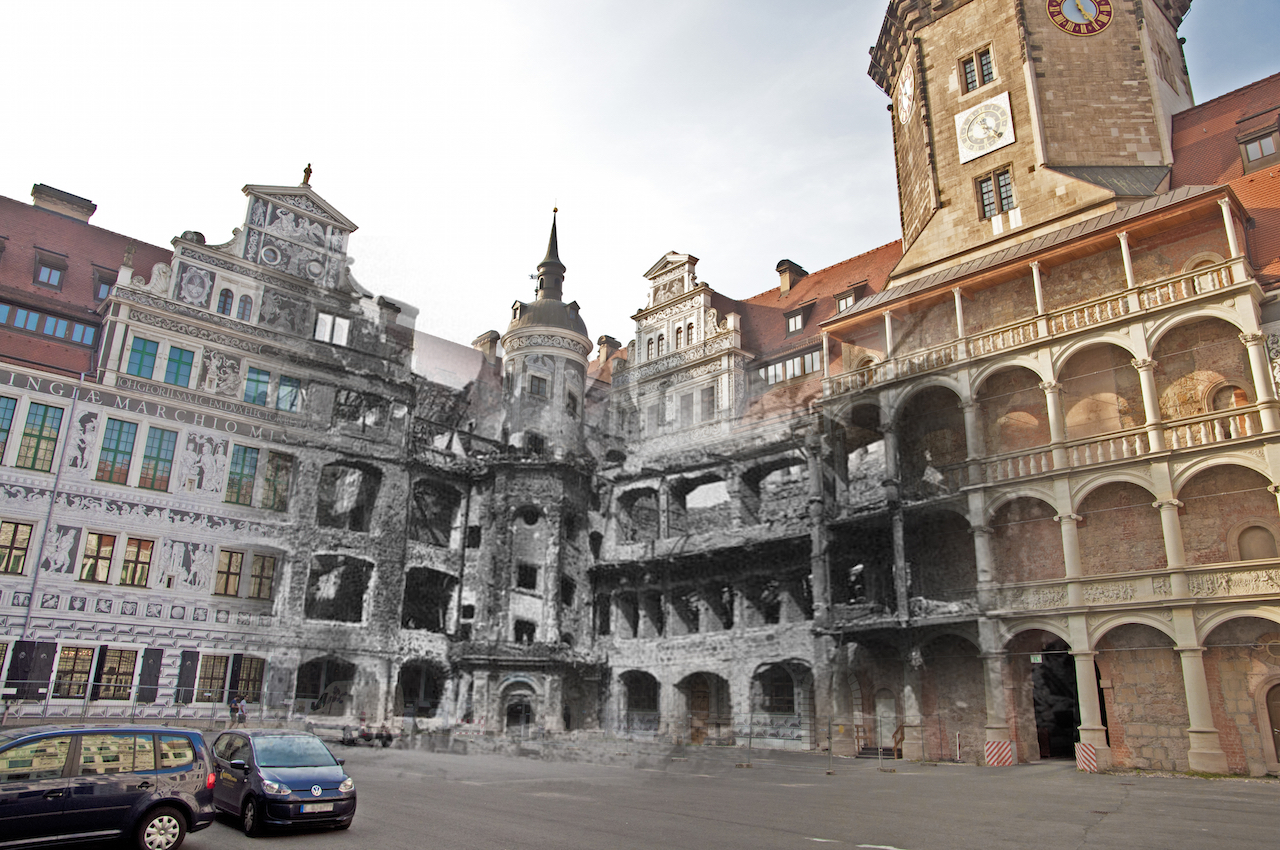
\includegraphics[width=\textwidth]{gfx/1945_2014_Residenzschloss_small.jpg}
   \caption[Rephoto of Dresden Castle]{Rephoto of the Dresden Castle, destroyed during World War II,
   \textcopyright\ Sergey Larenkov, printed with permission}
   \label{fig1}
\end{figure}

\begin{figure}
   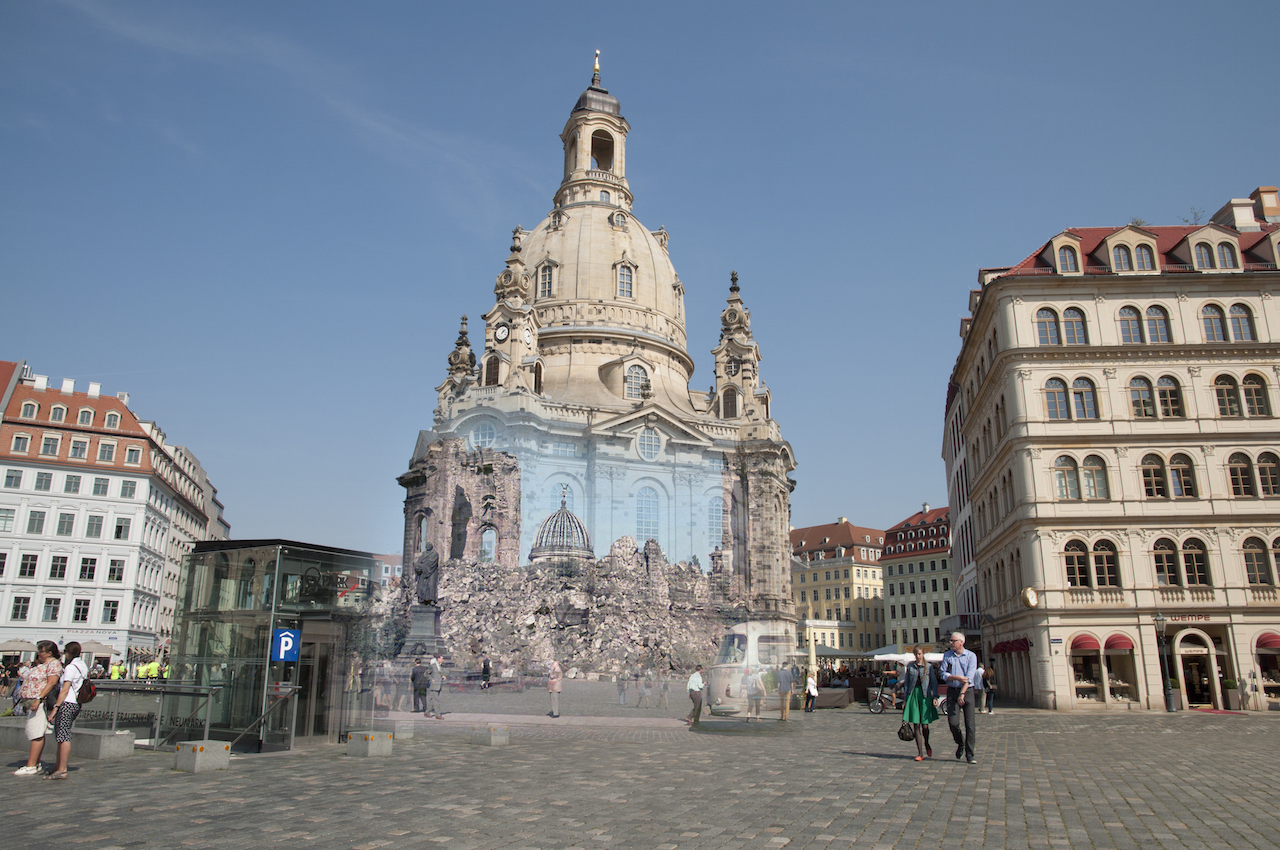
\includegraphics[width=\textwidth]{gfx/1950_2014_Frauenkirche_small.jpg}
   \caption[Rephoto of Dresden Frauenkirche]{Rephoto of the Dresden Frauenkirche, destroyed during World War II,
   \textcopyright\ Sergey Larenkov, printed with permission}
   \label{fig2}
\end{figure}

When done manually, the photographer must attempt to find the original viewpoint 
usually by visual inspection of the original image and trying to match the
current camera parameters---camera position, camera rotation, focal length,
possibly principal point---to the original.
The procedure is often carried out by placing the camera on a tripod and
comparing a printout of the original image with what can be seen through the
viewfinder or the camera screen. The number of parameters to match as well as
the difficulty to estimate them purely from comparing two-dimensional images makes the process
error-prone and tedious. Visual acuity and experience of the photographer thus
place limits on the accuracy with which the camera pose of the reference image
can be reconstructed. Some corrections can be done by post-processing the images
and warping the rephotograph with a homography to better match the original, but
it would be preferable to achieve a good result in-camera.

At the time of writing, few computerised aids are available to the photographer
(see \autoref{subsec:mobile_apps}).  The advancement of mobile phones and tablet
computers with integrated cameras and larger screens presents the opportunity to
develop applications which can assist in this endeavour, moving away from the
traditional trial-and-error approach.  On current digital cameras\footnote{At
   the time of writing, no commercial manufacturer produces a camera with
   user-modifiable firm- or software. A project at Stanford by \citet{Levoy2010}
was discontinued \citep{FrankenCam}.} this is impossible due to their closed
infrastructure not permitting to run user programs. 

\section{Previous Approaches To Assisted Rephotography}

\subsection{Mobile Applications}\label{subsec:mobile_apps}

Two applications have been developed to assist a photographer in taking
rephotographs. For smartphone operating systems,
\emph{rePhoto}\footnote{\url{http://projectrephoto.com/}} and
\emph{Timera}\footnote{\url{http://www.timera.com/Explore}} exist, both
available for Android and iOS devices. These applications support the user by placing a transparent
version of the original image over the current camera image, allowing for easier
alignment. 
Both apps present the captured rephoto with the original image blended in, but
only Timera allows for customisation (see \autoref{fig:timera})

\begin{figure}
   {\centering      
      \fbox{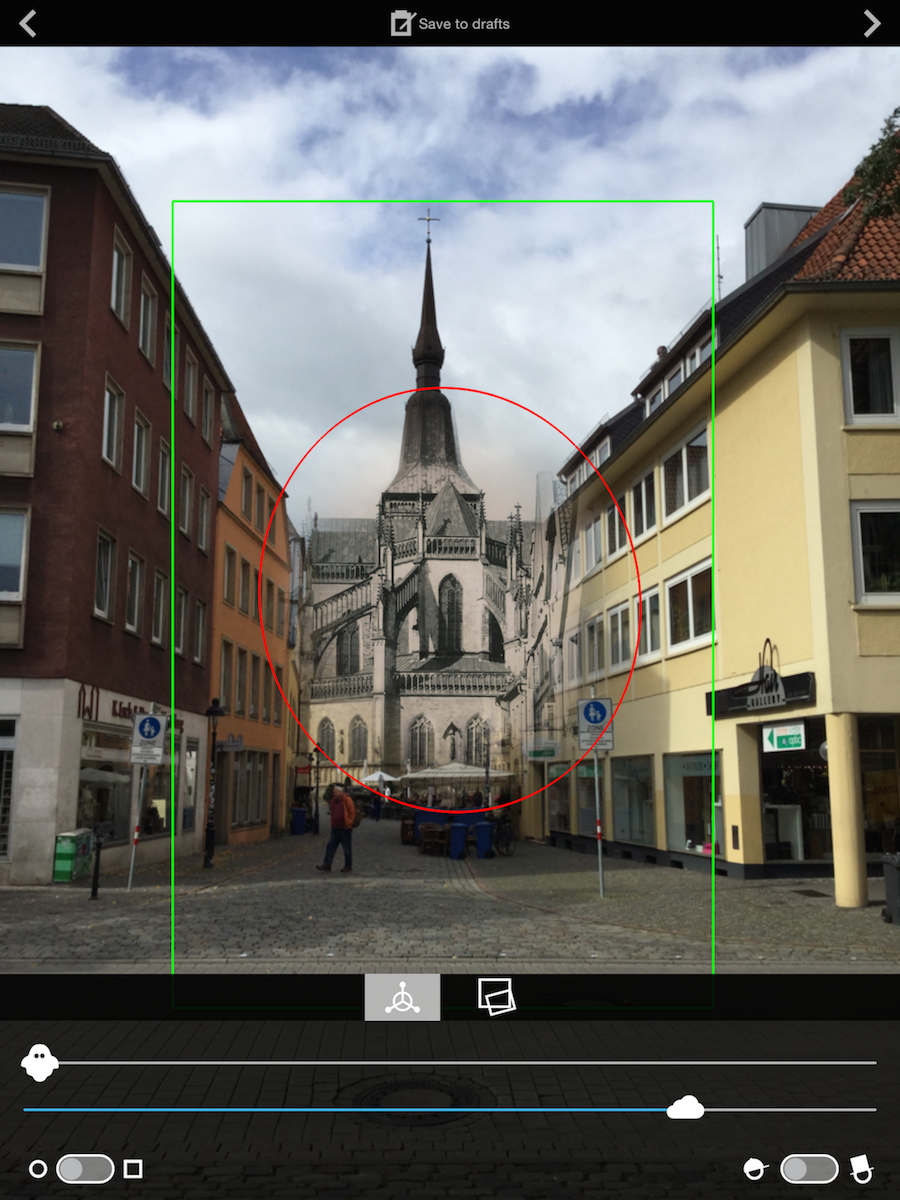
\includegraphics[width=.5\textwidth]{gfx/timera.PNG}}
      \caption[Overlay customisation with Timera]{Timera allows to select opacity,
      blend fuzziness and the portion of the old images that is visible.}
   \label{fig:timera}}
\end{figure}

What is characteristical about both of these applications is that the user must still
determine on their own how to actually move the camera. An overlay simplifies
the procedure, eliminating some of the inaccuracy introduced into the manual approach by the
necessity to move the eyes from printout to camera, but it is still the user's
responsibility to determine the necessary motion between the current camera
position and the goal position (that of the original image). 

\subsection{Computational Re-Photography}

A more sophisticated automated approach was presented by \citet{bae2010}. They
found in preliminary studies that neither a side-by-side view, as would be used
in the manual approach, nor a linear blend provided by the above applications
result in accurate rephotographs. Their design applies image processing and
geometrical reconstruction of the scene in order to guide the user into the right direction.

This
subsection will give a brief overview, while a more in-depth discussion of the
relevant concepts is deferred to \autoref{sec:app_challenges}. 
In this set-up, the relevant parameters of a historic image's camera are
reconstructed, including the focal length, principal point and the six degrees
of freedom in camera pose with structure-from-motion (SfM) techniques. Five problems
are addressed by \citet{bae2010}.

\begin{enumerate}
   \item It is difficult to communicate a necessary motion to the user if it has
      six degrees of freedom.
   \item While it is possible to compute the direction of translation between
      two camera frames given some corresponding points, its scale is unknown so
      that one does not know how far to move.
   \item As the translation between two camera frames becomes small, the
      estimate of relative translation becomes unstable.
   \item Historic images are visually very different from current ones, so that
      automatic feature detection will not work to obtain corresponding points.
   \item The historic images' camera is unknown, but its calibration parameters
      (see \autoref{subsec:intrinsics}) are needed.
\end{enumerate}

To ease the user's task and remove problem 1., \citet{bae2010} warp the current camera image
according to the camera rotation between the current camera frame and reference image.  The
user can then focus on correctly translating the camera. 

To solve the other problems, user interactions is required. The user captures
two frames of the scene with a wide baseline. Manual selection of some
correspondences between the historic image and one of the two just taken
eliminates the fourth problem, while the second one can be addressed by using
the two images and the current camera frame for 3D reconstruction. The fifth
problem is eliminated by estimating the unknown parameters after 
identifying some lines in the image which are parallel in reality.

The software runs on a laptop connected to a digital camera. On the computer
screen, the user is shown the current camera image alongside two arrows
indicating in which direction to move---one for movement in the sensor plane and
one for movement along the optical axis.

The results of this method appear to be very successful, but two main drawbacks
exist.

\begin{itemize}
   \item The prototype is not very convenient, as it requires a (laptop)
      computer and a digital camera which is impractical for
      spontaneous rephotography.
   \item The application is not available to the public, neither in source nor
      binary form. It is therefore impossible to evaluate or adapt for more mobility.
\end{itemize}

\section{Goals of this thesis}

This work's objective can thus be summarised as follows.
\begin{enumerate}
   \item Implement in a prototypal fashion the process from \citep{bae2010} for
      a mobile operating system so it can be run on a smartphone or tablet and
      direct the user in approximate real-time.
   \item Evaluate the approach and attempt to reproduce the results.
\end{enumerate}

For a proof-of-concept application, several simplifying assumptions are made.
Firstly, it is assumed that the ``historic'' photograph is captured with the
same camera as the one running the application and that the camera is calibrated.
Secondly, no strong visual differences between the reference and current scenes
are assumed so that the reference image is accessible to the same feature
detection algorithm without the user manually labelling correspondences. This
entails that the procedure will not work on historic images, but the extension
is relatively straightforward.

The application targets iOS 8 and current hardware, as image processing is
computationally intense, and has been tested on an iPad Air 2.


\chapter{Camera Geometry}

This chapter will introduce the geometry of image projection, largely following
\citep[chapters 6,7]{h&z2004} and the geometry of two views (the epipolar
geometry, \citet[ch. 5.1]{ma2003}) and
how it can be used to recover relative camera position from two images of the
same scene. 

\section{Camera Models}

The camera model used is the ideal pinhole camera model which postulates several
idealised assumptions.
\begin{enumerate}
   \item The aperture size is infinitely small
   \item There are no lens effects (\emph{thin lens} assumption)
   \item The angle of view is arbitrarily large
   \item All world points projected onto the image plane are in focus, owing to
      the small aperture
\end{enumerate}


Given a camera $C$ whose centre of projection is the origin and a point
$\mbf{X}$ in camera-centric coordinates, the central projection of
$\mbf{X}$ onto $C$'s image plane is depicted in a side-view in
\autoref{pinhole}.  The image plane is virtually moved to the front of the
camera, otherwise the image would be mirrored at the principal point as in real
cameras.  Let $f$ be the focal length, which is the distance of the image plane
to the optical centre.  If $\mbf{X} = (X,Y,Z)$, then $x=\left(f \frac{X}{Z},
f \frac{Y}{Z}, f\right)$ by use of the intercept theorem.%, with $\left(fX, fY\right)^T$ being the coordinates in the image plane.


\begin{figure}[h]
   {\centering      
      \begin{tikzpicture}[every node/.style={outer sep=0,inner sep=0},
   label distance=5pt]
   \usetikzlibrary{calc}
   \fill (0,0) circle (2pt) node[label=below:{$C$}] (C) {};
   \draw[->,name path=y-axis] (C) -- ++(0,4cm);
   \draw[->,name path=x-axis] (C) -- ++(8cm,0);

   \fill (7cm,3cm) circle (2pt) node[label=above right:{$\mathbf{X}$}] (X) {};

   \draw[name path=image plane] (3cm,1.7cm) -- ++(0,-2*1.7cm);

   \draw[|-|] (0,-2cm) -- (3cm,-2cm) node[midway,below=1em] (f) {$f$};

   \draw[name path=ray] (C) -- (X);
   \fill[name intersections={of=ray and image plane}]
   (intersection-1) circle (2pt) coordinate (c);
   \node[label=above left:{$x$}] (x) at (c) {};

   \draw[dashed] (0,3cm) node[left=1em] {$Y$} -- (X) -- (7cm,0)
   node[below=1em]
   {$Z$};

   % \draw[|-|] (0,-3cm) -- (7cm,-3cm) node[midway,below=1em] (Z) {$Z$};

   \draw[|-|,name intersections={of=x-axis and image plane}] (x) ++(1em,0) --
   ($(intersection-1) + (1em,0)$) node [right=1em,midway] {$f \cdot
   \frac{Y}{Z}$};

\end{tikzpicture}

      \caption{Central projection for a pinhole camera}
   \label{pinhole}}
\end{figure}


When representing the points as homogeneous\footnote{Homogeneous vectors are
the elements of projective geometry. They can be obtained from Cartesian
coordinates by appending a 1-element. All projective entities which differ only
by a scalar factor are equivalent, one writes $\mbf{x} \sim \mbf{y}$ if
$\mbf{x} = \lambda\mbf{y}, \lambda \neq 0$. This has the added effect that
points at infinity can be represented by vectors whose last coordinate is zero.} 
quantities, the central projection
can be expressed by a matrix multiplication. 
This can be written with homogeneous coordinates as
\begin{IEEEeqnarray}{rCl} \label{eq:projection}
      \left(
         \begin{array}{c}
            fX \\ fY \\ Z
         \end{array}
      \right) & = & \underbrace{\addstackgap[6pt]{\left(
         \begin{array}{cccc}
            f & 0 & 0 & 0 \\
            0 & f & 0 & 0 \\
            0 & 0 & 1 & 0
         \end{array}
\right)}}_{\text{Projection Matrix of $C$}} \left(\begin{array}{c} X \\ Y \\ Z \\ 1 \end{array}\right)
\end{IEEEeqnarray}
or in short
\begin{equation}
   \mbf{x} \sim P\mbf{X}
\end{equation}

% If the unit of the coordinate system is chosen to be $f$, then the image plane is
% $Z = f$ and 
% \eqref{eq:projection} becomes
% \begin{IEEEeqnarray}{rCl}
%       \left(
%          \begin{array}{c}
%             X \\ Y \\ \frac{z}{f}
%          \end{array}
%       \right) & = & \addstackgap[6pt]{\left(
%          \begin{array}{cccc}
%             1 & 0 & 0 & 0 \\
%             0 & 1 & 0 & 0 \\
%             0 & 0 & \frac{1}{f} & 0
%          \end{array}
% \right)} \left(\begin{array}{c} X \\ Y \\ Z \\ 1 \end{array}\right)
% \end{IEEEeqnarray}

\subsection{Camera Extrinsics}

The above situation is a special case wherein the camera centre $C$ defines the
origin and the optical and image axes are the coordinate axes. Thus, the rotation
and translation of the camera relative to this coordinate system is zero. More
generally, there might be a world coordinate frame with different origin 
and different axes, so that a coordinate transform must be applied to $\mbf{X}$
before the projection. 

Let $R \in \mathbb{R}^{3\times3}$ be a rotation matrix
giving the camera's rotation relative to the world frame and $t \in
\mathbb{R}^{3\times1}$ its translation such that

\begin{equation}
   \mbf{X}_{\text{cam}} = R \mbf{X}_{\text{world}} + t
\end{equation}

Then the projection of a point $\mbf{X}$
in world coordinates onto the image plane becomes

\begin{IEEEeqnarray}{rCl}\label{eq:projection_rt}
   \mbf{x} & = & P \mbf{X}\\
   \mbf{x} & = & \left(\begin{array}{ccc}
   f & 0 & 0 \\
   0 & f & 0 \\
   0 & 0 & 1
   \end{array}\right) \left[R \mid t\right] \mbf{X}
\end{IEEEeqnarray}

\subsection{Camera Intrinsics}
\label{subsec:intrinsics}

Most cameras are not pinhole cameras. To make them conform to the model, the
camera intrinsics need to be known.  Above, the resulting image points $\mbf{x}$
were in \emph{normalised} image coordinates. In particular, the principal
point---the intersection of the image plane with the optical axis---was assumed
to be $(0,0)$. But generally, image coordinates are expressed in pixels relative
to the upper left corner of the sensor. To convert between normalised and pixel
coordinates, the camera's five intrinsic parameters and can be written in matrix
form and premultiplied in \eqref{eq:projection_rt} as
\begin{IEEEeqnarray}{rCl}
   \mbf{x} & = & \left(
   \begin{array}{ccc}
      s_x & s     & c_x \\
      0   & s_y   & c_y \\
      0   &       & 1
   \end{array} 
\right) \left(\begin{array}{ccc}
   f & 0 & 0 \\
   0 & f & 0 \\
   0 & 0 & 1
\end{array}\right) \left[R \mid t\right] \mbf{X}
\end{IEEEeqnarray}
where $s_x$ and $s_y$ are the focal lengths in $x$- and $y$-directions expressed
in pixel units per world unit (e.g. cm; $s_x$ and $s_y$ are not necessarily identical, if the sensor has
non-square pixels), $s$ the sensor skew (the pixels may not be rectangular;
their edges may not be perpendicular) which is usually zero, and the coordinates
of the principal point $(c_x,c_y)$ with respect to the origin of the image plane
which usually placed at the upper left corner.
The intrinsic camera parameters are assembled in
\begin{IEEEeqnarray}{rCl}
   K & = & \left(\begin{array}{ccc}
   fs_x & s & c_x \\
   0 & fs_y & c_y \\
   0 & 0 & 1
\end{array}\right)  
\end{IEEEeqnarray}
are therefore essential to
relate world points to image points which will be important for this
application. The normalised coordinates $\hat{\mbf{x}}$ for a pixel coordinate
$\mbf{x}$ can be computed as
\begin{equation}
   \hat{\mbf{x}} = K^{-1}\mbf{x},
\end{equation}
which will remove the effects of the calibration parameters and thus make the
image coordinates independent of the camera's internal characteristics.

In theory, these parameters could be obtained from the camera's
vendor who knows the precise manufacturing specifications. In practice, only the
focal lengths $f_x, f_y$ are known, in most cases only one with the assumption
of square pixels. Usually, the principal
point is assumed to be at the sensor centre and the pixels are assumed to be
rectangular. In practice however, there are variances introduced by different
causes such as imprecise manufacturing or physical impacts which may decentre
the lens such that the principal point is no longer at the centre. 

A further complication is introduced by the camera lens which will often have a
non-negligible distortion, most prominently radial distortion as depicted in
\autoref{distortion}, but the thin lens assumption precludes distorted images.  It
can be modelled by the application of a distortion factor to the ideal
undistorted image coordinates $(\tilde{x}, \tilde{y})$
and thus removed to satisfy the thin lens assumption. Distorted an ideal image
coordinates are related as
\begin{equation}
   \begin{pmatrix}
      x_d \\ y_d
   \end{pmatrix} = L(r)\begin{pmatrix}
      \tilde{x} \\ \tilde{y}
   \end{pmatrix}
\end{equation}

\begin{figure}
   {\centering      
      \begin{tikzpicture}[every to/.style={color=red}]

   \makegrayinprint

   \newcommand{\yshift}{6cm}
   \draw (0,0) rectangle (4,3);
   \begin{scope}[xshift=2cm,yshift=1.5cm]
      \draw (-1.5,-1) to[bend right=8] (1.5,-1) to[bend right=8] (1.5,1) to[bend
      right=8] (-1.5,1) to[bend right=8] (-1.5,-1);
   \end{scope}
   \begin{scope}[xshift=\yshift]
      \draw (0,0) rectangle (4,3);
      \begin{scope}[xshift=2cm,yshift=1.5cm]
         \draw (-1.5,-1) to (1.5,-1) to (1.5,1) to (-1.5,1) to (-1.5,-1);
      \end{scope}
   \end{scope}
\draw[-{Latex},thick,color=RoyalBlue,text=black] (4,1.5) ++(1mm,0) -- node[below,midway,font=\footnotesize]
   {correction} ($(\yshift,1.5) - (1mm,0)$);
\end{tikzpicture}

      \caption[Radial distortion]{Radially distorted image on the left, the corrected image on the
   right.}
   \label{distortion}}
\end{figure}

where $L$ is a nonlinear function of the distance $r$ from the distortion
centre---usually coincident with the principal point. The function can be
approximated as an exponential with a Taylor expansion
\begin{equation}
   L(r) = 1 + \sum\limits_{i=1}^k \kappa_i r^i
\end{equation}
for a given $k$ \citep[see][ch. 7.4]{h&z2004}. The intrinsic camera
parameters which consist in the entries of $K$ and distortion coefficients
$\kappa_i$ must be determined in order to accurately relate world coordinates to
image coordinates. They can be found by calibrating the camera. Different
methods exist \citep[e.g][]{zhang2000} but will not be examined here.

\section{Epipolar Geometry}
\label{sec:epipolar}

Epipolar geometry is the geometry which relates the image points in two views of
the same scene. \autoref{epipolar} shows the basic set-up. 

We consider a scene viewed by two cameras with optical centres $c_1$ and $c_2$,
where $c_1$ defines the origin,
world points $\mbf{X}_i\in\mathbb{R}^3$, where the subscript denotes the coordinate
frame---the first camera, arbitrarily chosen to be the left one, or the second
camera---and homogeneous image points $\mbf{x}_i$ which are the projections of $\mbf{X}_i$
onto the image planes and thus correspond to the same world point. The cameras
are related by a rigid body transform $(R,T)$, where $R$ is a $3\times3$
rotation matrix and $T$ the translation between the camera centres. Throughout
this work, the direction of coordinate frame transformation will be such that
\begin{equation}\label{eq:camera_transform}
   \mbf{X}_2 = R\mbf{X}_1 + T.
\end{equation}

It is obvious that the following relation holds,
\begin{equation}\label{eq:project_world_point}
   \lambda_i\mbf{x}_i = \mbf{X}_i, ~\lambda_i > 0
\end{equation}
that is, the world point lies on a ray through the optical centre and the image
point. 

\begin{figure}[h]
   {\centering      
      \usetikzlibrary{intersections, calc, arrows.meta}
\begin{tikzpicture}[every node/.style={outer sep=0,inner sep=0},
   label distance=5pt]
   \def\baseline{10cm}
   \draw[fill] (0,0) circle (2pt) node[label=below left:{$c_1$}] (c1) {};
   \draw[fill] (\baseline,0) circle (2pt) node[label=below left:{$c_2$}] (c2) {};

   \newcommand{\sensorplane}[1]{
      \path[name path=#1,draw] (1cm,0.5cm) -- (1cm,2.5cm) -- (3.5cm,1cm) -- (3.5cm,-1cm) -- cycle
   }
   \begin{scope}
      \sensorplane{plane1};
   \end{scope}

   \begin{scope}[yscale=1,xscale=-1,xshift=-\baseline]
      \sensorplane{plane2};
   \end{scope}

   \fill (0.5*\baseline,3cm) circle (2pt) node[label=above:{$\mathbf{X}_1$}]
   (X1) {};

   \draw (c1) -- ++(3cm,0) [fill] circle (2pt) node[label=above:{$e_1$}] (e1)
   {} coordinate (c);
   \draw[dotted] (c) -- (3.5cm,0) coordinate (c);
   \draw[solid] (c) -- (\baseline-3.5cm,0) coordinate (c);
   \draw[dotted] (c) -- (\baseline-3cm,0) coordinate (c);
   \draw[fill] (c) circle (2pt) node[label=above:{$e_2$}] (e2) {} -- (c2);

   % lines from camera center to x
   \path[name path=c1 to X1] (c1) -- (X1) coordinate[pos=.3] (c);
   \draw[solid,fill] (c1) -- (c) coordinate (x1) circle (2pt);
   \node[label=above:{$x_1$}] (x1) at (c) {};
   \draw[dotted,name intersections={of=c1 to X1 and plane1}] (c) --
   (intersection-2) coordinate (c);
   \draw[solid] (c) -- (X1);

   \path[name path=c2 to X1] (c2) -- (X1) coordinate[pos=.3] (c);
   \draw[solid,fill] (c2) -- (c) coordinate (x2) circle (2pt);
   \node[label=above:{$x_2$}] (x2) at (c) {};
   \draw[dotted,name intersections={of=c2 to X1 and plane2}] (c) --
   (intersection-2) coordinate (c);
   \draw[solid] (c) -- (X1);

   % draw epilines
   \draw[RoyalBlue,text=black] (e2) -- (x2) node[midway,label=above:{$l_2$}] (label-l2) {};

   \draw[RoyalBlue,text=black] (e1) -- (x1) node[midway,label=above:{$l_1$}] (label-l1) {};

   % draw relative rotation and translation
   \draw[-{Latex}] ($(c1) + (2em,-2em)$) to[bend right=50] node[below=1em, midway]
   {$R$, $T$} ($(c2) + (-2em,-2em)$);

\end{tikzpicture}

      \caption[Basic epipolar geometry]{Basic epipolar geometry with camera centres $c_1$, $c_2$, image
      points $\mbf{x}_1$, $\mbf{x}_2$, a world point $\mbf{X}_1$, epipoles
   $e_1$, $e_2$ and epipolar lines $l_1$, $l_2$}
   \label{epipolar}}
\end{figure}

Given the corresponding points $\mbf{x}_i$ in two images, the ultimate goal is
to retrieve the euclidean transform $(R,T)$.

In case the image coordinates for both cameras are normalised (c.f.
\autoref{subsec:intrinsics}), they have equal units, so
starting from \eqref{eq:camera_transform}, one can derive
\begin{IEEEeqnarray*}{rClls}
   \mbf{X}_2 & = & R\mbf{X}_1 + T & \hspace {2cm} \\
   \lambda_2\mbf{x}_2 & = & R\lambda_1\mbf{x}_1 + T & & (by \eqref{eq:project_world_point}) \\
   \lambda_2\widehat{T}\mbf{x}_2 & = & \widehat{T}R\lambda_1\mbf{x}_1 + \widehat{T}T & &
   $\widehat{T}\in\mathbb{R}^{3\times3}$ with $\widehat{T}\mbf{x} = T \times
   \mbf{x}$ \\
   \lambda_2\mbf{x}_2^T\widehat{T}\mbf{x}_2 & = &
   \mbf{x}_2^T\widehat{T}R\lambda_1\mbf{x}_1 + 0 & & $T \times T = 0$ \\
   \lambda_2\cdot 0 & = &
   \mbf{x}_2^T\widehat{T}R\lambda_1\mbf{x}_1 & & $\widehat{T}\mbf{x}_2$ is
   perpendicular to $\mbf{x}_2$ \\
   0 & = & \mbf{x}_2^T\underbrace{\widehat{T}R}_{E}\mbf{x}_1
   \label{eq:epiconstraint}\IEEEyesnumber
\end{IEEEeqnarray*}

The product $E=\widehat{T}R$ is the \emph{essential matrix} and the constraint it
imposes on corresponding image points the \emph{essential constraint}
\citep[see][ch. 5]{ma2003}. 

An intuition for the essential matrix can be
obtained from \autoref{epipolar}. Given an image point in one frame $\mbf{x}_1$,
in attempting to find the point $\mbf{x}_2$ corresponding to the same world
point $\mbf{X}_1$, the epipolar geometry restricts the search space to one
dimension---the epipolar line of $\mbf{x}_1$ in the second camera's image plane.
The camera centres and the world point define an epipolar plane. The
backprojection of $\mbf{x}_1$ is the ray through $\mbf{x}_1$ and the optical
centre $c_1$. All points on this ray are mapped to the same point on the image
plane of $c_2$. Depending on how far away the world point $\mbf{X}_1$ is from $c_1$, its
image on the second camera's image plane will vary---but it will be on the
intersection of the image plane and the epipolar plane, the epipolar line of
$\mbf{x}_1$. The line $l_2$ may be identified with its coimage (the orthogonal
complement of its preimage) $l_2 = e_2 \times \mbf{x}_2 \in \mathbb{R}^3$ so that

\begin{equation} \label{eq:epiline}
   \forall\mbf{x}: \mbf{x}\in l_2 \Leftrightarrow \mbf{x}\cdot l_2 = 0.
\end{equation} 

The coimage of the epipolar line is the vector perpendicular to the epipolar plane,
so every vector in this plane will have an inner product of $0$ with this
vector. Constrained to vectors in the image planes, this means that all vectors on the
epipolar line will have an inner product of $0$ with this vector $l_2$.
Referring back to \eqref{eq:epiconstraint}, it can be seen that multiplication
with $E$ will yield a term $\mbf{x}_2^TE = l_2$ which fulfils 
\begin{equation}
   \mbf{x}_1 \cdot l_2 = 0,
\end{equation}
which is precisely the relation stated in \eqref{eq:epiline}. The essential
matrix thus maps an image point onto its epipolar line in the other image.

\section{Essential Matrix Estimation}

Estimating the essential matrix between two
cameras and decomposing it into relative rotation and translation is a necessity
in the endeavour to communicate a necessary camera movement to the application's
user. The most prominent algorithms in this regard are the 8-Point algorithm
introduced in its original form by \citet{longuet-higgins1987} and improved upon
by \citet{hartley1997}, and the 5-Point algorithm proposed by
\citet{nister2004}. To illustrate the mathematical tractability of the problem,
the former will be presented below.

\subsection{The 8-Point Algorithm}\label{sec:eight-point}

The essential matrix has nine elements, but since all image coordinates are
projective quantities, the set of all essential matrices differing by a constant
factor is equivalent so that one degree of freedom is removed and at most eight
remain. If one were to formulate constraints on the elements as a system of
linear equations, eight of those should be sufficient to uniquely determine an
essential matrix. An improvement suggested in \citep{hartley1997} is the
preprocessing of the input data (the image coordinates) by translation and
scaling. This improves the robustness of the algorithm, but will be omitted
here.

For each point correspondence $\{\mbf{x}_1 = (x_1^i,y_1^i,1),\mbf{x}_2 = (x_2^i, y_2^i,
1)\}$, one linear equation
\begin{equation}
   \mbf{x}_2^T E \mbf{x}_1 = 0
\end{equation}
is generated, which can be rewritten as
\begin{IEEEeqnarray*}{rCcCcCc}
   0 & = & x_2^i x_1^i e_{11} & + & x_2^i y_1^i e_{12}  & + &  x_2^i e_{13} \\
     & + & y_2^i x_1^i e_{21} & + & y_2^i y_1^i e_{22} & + & y_2^i e_{23} \\
     & + & x_1^i e_{31} & + & y_1^i e_{32} & + & e_{33} \label{eq:linear_equation}
   \IEEEyesnumber
\end{IEEEeqnarray*}
Let $\mbf{e}$ denote the vector of $E$'s entries in row-major order, then
\begin{equation}
   0 = \left( x_2^i x_1^i, x_2^i y_1^i, x_2^i, y_2^i x_1^i, y_2^i y_1^i, y_2^i, x_1^i, y_1^i,
   1\right)\cdot\mbf{e}
\end{equation}

If $n$ correspondences are given, they each contribute one row to
\begin{IEEEeqnarray}{rCl}
   A\mbf{e} & = & \left[ \begin{array}{ccccccccc}
      x_2^1 x_1^1 & x_2^1 y_1^1 & x_2^1 & y_2^1 x_1^1 & y_2^1 y_1^1 & y_2^1 & x_1^1 & y_1^1 & 1 \\
   \vdots & & & & & & & & \vdots \\
      x_2^n x_1^n & x_2^n y_1^n & x_2^n & y_2^n x_1^n & y_2^n y_1^n & y_2^n & x_1^n & y_1^n & 1
\end{array} \right] \mbf{e} = 0 \nonumber\\*\label{eq:stacked_essential}
\end{IEEEeqnarray}

\newcommand{\norm}[1]{\left\lVert#1\right\rVert}

For eight noise-free point correspondences in non-degenerate general position, there is a
unique solution (up to scale) besides the trivial zero, but in practice, one
uses more correspondences and the system is overdetermined, so a
least-squares-solution minimising $\norm{ A\mbf{e} } = \sum_{ij}
(A\mbf{e})_{ij}^2$ is sought.  The solution is unique up to scale, since all
multiples of $\mbf{e}$ will satisfy \eqref{eq:stacked_essential}---this is also
the reason why the scale of the translation cannot be determined. One therefore
introduces the constraint $\norm{ \mbf{e} } = 1$ which also excludes a trivial
zero solution.

This solution vector is the singular
vector with the smallest singular value in the singular value decomposition of
$A$ or equivalently, the eigenvector of $A^TA$ with the smallest eigenvalue
\citep[see][]{hartley1997}.

\subsection{Further Algorithms}

The 8-Point Algorithm is mathematically straightforward and linear, but in
practice it suffers from noise \citep[see][]{luong1993} and in real
applications approaches the robustness of other methods only in its normalised
form from \citep{hartley1997} (not related to \emph{normalised image
coordinates}).

It has been noted above that $E$ can have at most eight degrees of freedom. In
reality, it has only five, as rotation and translation have three degrees of
freedom each, and one is lost due to the indeterminable scale. In theory five
constraints from five pairs of image points thus are sufficient for finding $E$.
A solution was put forth by \citet{nister2004}, improved in
\citep{stewenius-engels-nister2006}. The algorithm is nonlinear and
thus much less easily understood and implemented, involving computing the roots
of a ten degree polynomial, and requires only five points, but can also be
applied to more. It can be considered a state-of-the-art solution to the
relative pose estimation problem; its performance in overdetermined cases in the
presence of noise compares favourably to other
direct methods requiring six \citep{pizarro2003}, seven or eight points.

Many other methods exist. Some---like the algorithms described above---find a
globally optimal solution in closed form---, while others employ heuristic
methods to iteratively approach a local optimum. A review is given in \citep{zhang1998}.

Direct methods such as the five-point or eight-point algorithms are frequently
used in schemes like RANSAC, which make the estimation more robust to outliers
(correspondences which are imprecise or incorrect). For a number of iterations,
a hypothesis for $E$ is computed on a minimal number of correspondences and then
evaluated on the whole data set. If the inliers in the data far outweigh the
outliers, it is probable that a noise-free subsample is selected. The best hypothesis is kept.
The simplified algorithm is shown in \autoref{alg:ransac}
\citep[c.f.][ch. 4.8]{h&z2004} and requires an error measure for $E$.


   \SetAlCapSkip{1ex}
\begin{algorithm}
   \caption{Simplified RANSAC scheme for essential matrix estimation}
   \label{alg:ransac}
   \KwData{$n$ point correspondences}
   \KwResult{a best-fitting essential matrix}
   Let $c_{\text{best}} \coloneqq 0$\;
   \For{$i \coloneqq 0$, $i < maxIter$}{
      Select randomly a minimal number of points to estimate $E_i$\;
      Compute error measure for $E_i$ on all $n$ points\;
      Let $C_i$ be the set of point pairs whose error does not exceed $\varepsilon$\;
      \If{$|C_i| > c_{\text{best}}$} {
         $c_{\text{best}} \coloneqq |C_i|$\;
         $E_{\text{best}} \coloneqq E_i$\;
      }
   }
   return $E_{\text{best}}$
\end{algorithm}

\section{Decomposing The Essential Matrix}

One step remains to recover the relative camera pose from corresponding points.
As per the derivation in \autoref{sec:epipolar}, the rotation and translation
between the two cameras is encoded in $E$. Given an essential matrix,
\citet[ch. 9.6]{h&z2004} show that there are four mathematically valid
decompositions of $E$ into $R$ and $T$, corresponding to four distinct
geometrical scenarios \citep[see][ch. 9.6]{h&z2004}. Only one of the
solutions will place a point $\mbf{X}_2 = R\mbf{X}_1 + T$ in front of both
cameras, the others cannot be realised in practice.  Triangulating one point
from its corresponding image points in the two views will therefore reveal the
one correct solution, with the translation scale unknown.


\chapter{Challenges In Relative Pose Estimation}

The success of recovery of relative pose mainly depends on two factors: The
accuracy and correctness of image point correspondences and them not being in a
degenerate configuration, so that an epipolar geometry can be estimated from
them.  This chapter will examine the preconditions and the feasibility of pose
recovery in realistic conditions. Several problematic cases will be identified
and described. Furthermore, an assessment of different feature detection
algorithms for the purpose of this work will be given.

\section{Degenerate Configurations}

Degenerate configurations are those in which the data on which the essential
matrix is estimated allows for more than one mathematically valid solution. Two
different cases can be observed.

\subsection{Structure Degeneracy}

Structure degeneracy is a configuration of points in the observed scene which do
not provide enough information to wholly determine an essential matrix. The
projection matrix $P\in\mathbb{R}^{3\times3}$ with 
\begin{equation*}
   \mbf{x} = P\mbf{X}
\end{equation*}
has twelve elements but is a projective quantity, so all non-zero multiples of
$P$ are equivalent, wherefore it has only eleven degrees of freedom.  A
degenerate case is for instance when all points observed by the two cameras lie
on the same plane (or worse, a subspace of even lower dimension). The images of
a planar surface in two cameras as well as the planar surface itself and its
image are related by a homography \citep[see][ch. 13]{h&z2004}, which is a
mapping between planes and has eight degrees of freedom (being a $3\times3$
matrix and a projective element), meaning that three degrees of freedom are
undetermined \citep{torr1999}. A set of coplanar points alone thus does not provide
enough information to uniquely determine an epipolar geometry.

However, not all algorithms are susceptible to this problem. While the 8-point
algorithm alone cannot deal with this case, the five-point algorithm can and is
generally more robust \citep{li2006}. While there are other approaches to work
around such issues (e.g. an algorithm developed by \citet{chum2005} or
\citet{decker2008}), in practice, a five-point algorithm in a RANSAC scheme
works well and needs fewer iterations than an 8-point approach \citep{li2006}.

\subsection{Motion Degeneracy}
\label{subsec:motion_degen}

A second type of degeneracy occurs when the camera motion between two images has
fewer degrees of freedom than the model to be estimated---the essential matrix.
If the camera only translates or only rotates between images, the motion has
maximally three degrees of freedom. As \citet{decker2008} point out, an
essential matrix estimated under such conditions could be consistent with all
correct point matches, but also with some false ones due to the mismatch in
degrees of freedom between data and model. In schemes like RANSAC, such an
estimate will have a large consensus set---all inliers \emph{plus}
outliers---and so may lead to the termination of the algorithm, despite being
inaccurate.

It is unlikely in rephotography that the observed scene will be completely
planar, or that the user will move from the first frame in a motion which is
pure rotation or translation, these degeneracies can be labelled edge cases and
are not specifically handled in the application.

However, the most degenerate case is the one with zero motion between the frames
and of primary importance for this application. An initial idea to simply
compare the original image with the current frame cannot be successful as
relative pose estimation from corresponding points becomes unstable when the
motion between the two cameras approaches zero. But this is the ultimate goal one
wishes to achieve. When na\"ivley comparing the current camera
image to the reference photograph, the estimate for relative rotation and
translation would become increasingly unreliable as the camera approaches the
original viewpoint.  

\section{Finding Correspondences}

There is a variety of automatic feature detection algorithms which differ in
repeatability, robustness to noise, speed and invariance with respect to image
characteristics such as scale, brightness, or rotation. 
Generally, a feature detector identifies potentially salient points in an image
and computes a descriptor for these points in a way that the same point under
different conditions will yield an ideally identical descriptor. When points of
interest---usually called \emph{keypoints}---are available in multiple images,
their descriptors can be compared and the best match according to some metric
can be selected for each keypoint. The matches found can then be used as
corresponding points for relative pose estimation.

Classical state-of-the-art detectors include e.g. \emph{Scale-invariant feature
transform} \citep{lowe1999}, \emph{Speeded-up robust features}
\citep{bay2006} which both compute real-valued descriptors. A natural criterion
for selecting the best matching keypoint for a given keypoint is the $L_2$-norm
of the difference of their descriptors, which is a relatively expensive
operation. While e.g. SURF improves performance over the computationally
demanding SIFT detector, the speed of matching can still present a bottleneck in
time-critical contexts. The proliferation of mobile devices with more economic
hardware increased the demand for faster detection and matching of features and
many solutions have been proposed. On the one hand, efforts have been made at
faster feature detection algorithms in general (such as SURF or FAST
\citep{rosten2005}), but most promising are those which compute binary instead
of real-valued descriptors. The matching of $n$ features between images is an
$\mathcal{O}(n^2)$ operation when done with brute force, thus often placing a
limit on the computational efficiency of the whole process. On real hardware,
floating point operations are generally less efficient when compared to integer
or binary arithmetic. While for real-valued descriptors $d_1,~d_2$ with size $n$,
an $L_2$-norm 
\begin{equation*}
   \sqrt{\sum_{i=1}^n (d_1^i - d_2^i)^2}
\end{equation*}
must be evaluated,
binary strings can be compared with the Hamming distance 
\begin{equation*}
   \sum_{i=1}^n d_1^i \otimes d_2^i   
\end{equation*}
which is much faster. These descriptors include but are not limited to BRIEF
\citep[Binary Robust Independent Elementary Features]{calonder2010}, ORB
\citep[Oriented BRIEF]{rublee2011} and FREAK \citep[Fast Retina
Keypoint]{ortiz2012}. While some invariances are sacrificed in favour of
performance (such as rotation invariance of BRIEF, corrected by ORB), they are
claimed to match the repeatability of SIFT and others for many use cases while
being much faster to compute and compare. Another recent development by
\citet{alcantarilla2013} are AKAZE features, building on and accelerating the
previously proposed KAZE detector \citep{alcantarilla2012}, also using binary
strings to describe feature points. This detector has been chosen for this work
as it offers significant speed improvements over SIFT or SURF while sacrificing
no quality in the tested scenarios (see \autoref{ch:evaluation})\footnote{SIFT
and SURF are both protected by US patents and cannot be used without a license
in a commercial application in this country.}.

\subsection{SIFT \& AKAZE}\label{subsec:sift_akaze}

The SIFT detector attempts to find keypoints by convolving an input image with
gaussian kernels of successively larger variance, thus building a stack of image
\emph{scales}. This process is repeated for several \emph{octaves}, each starting
from a downsampled version of one of the blurred images from the previous scale
octave. The resulting pyramid is termed \emph{scale space}.  From these gaussian
images, difference-of-gaussians are computed by subtracting neighbours in scale
space. These difference images approximate an application of the Laplacian of
Gaussian (a Laplacian filter with prior smoothing to remove noise) which computes
the second spatial derivatives of the image and whose extremes are locations of
rapid intensity change like edges or corners. Within this scale space, extrema
are found which are such pixels in the DOG images whose absolute values are
maximal or minimal in comparison with their twenty-six neighbours in scale
space. This search is conducted in all DOG images for all octaves which
contributes to the scale invariance. After locating the keypoint with subpixel
accuracy in the image, keypoints are discarded if their absolute DOG value is
below some threshold as those are unstable and unlikely to be found under
differenc conditions. Furthermore, the Hessian of the
image (the matrix of second-order partial derivatives of the image intensity
function) is computed to filter out keypoints on edges as they are not accurately
localised and thus likewise unstable. Descriptors are computed by assigning a
primary orientation after analysing the intensity gradients in the region around the
keypoint and binning them into histograms. A keypoint's coordinate system is
rotated according to this primary orientation, thus achieving rotation
invariance. The resulting descriptor has 128 elements which will occupy at least
as many bytes.

In contrast to SIFT, where the scale space construction is linear since
convolution is linear, the scale space in AKAZE is nonlinear. Gaussian blurring
(a form of isotropic diffusion) at successively higher scale smooths not only
noise, but also true object boundaries which decreases the accuracy of
localising keypoints. A nonlinear scale space blurs the image in a way that
respects the local image structure and thus preserves object boundaries while
smoothing out noise. A visualisation of the difference is shown in
\autoref{fig:lin_vs_nonlin_diffusion}. The diffusion is large in homogeneous
areas and small in areas of significant intensity change.  A nonlinear scale
space is built for AKAZE by means of fast explicit diffusion
\citep{grewenig2010} and the diffusivity is adapted by considering the magnitude
of the image gradient at a given point---meaning that it will be smaller for
areas of strong change and larger for others. As in SIFT, the scale space
consists of several octaves, each downsampled by two with respect to the
previous octave. Within the ocataves, the images are called \emph{sublevels}.
The Hessian matrix determinant is used to identify possible keypoints (in SIFT,
this is used to filter out bad candidates),  but the candidate must be extremal
compared to other keypoint candidates in its neighbourhood instead of
neighbouring pixels. The window searched depends on the scale at which the
keypoint is located (the window is larger at higher scales with more blur).

\begin{figure}[h]
   {\centering      
      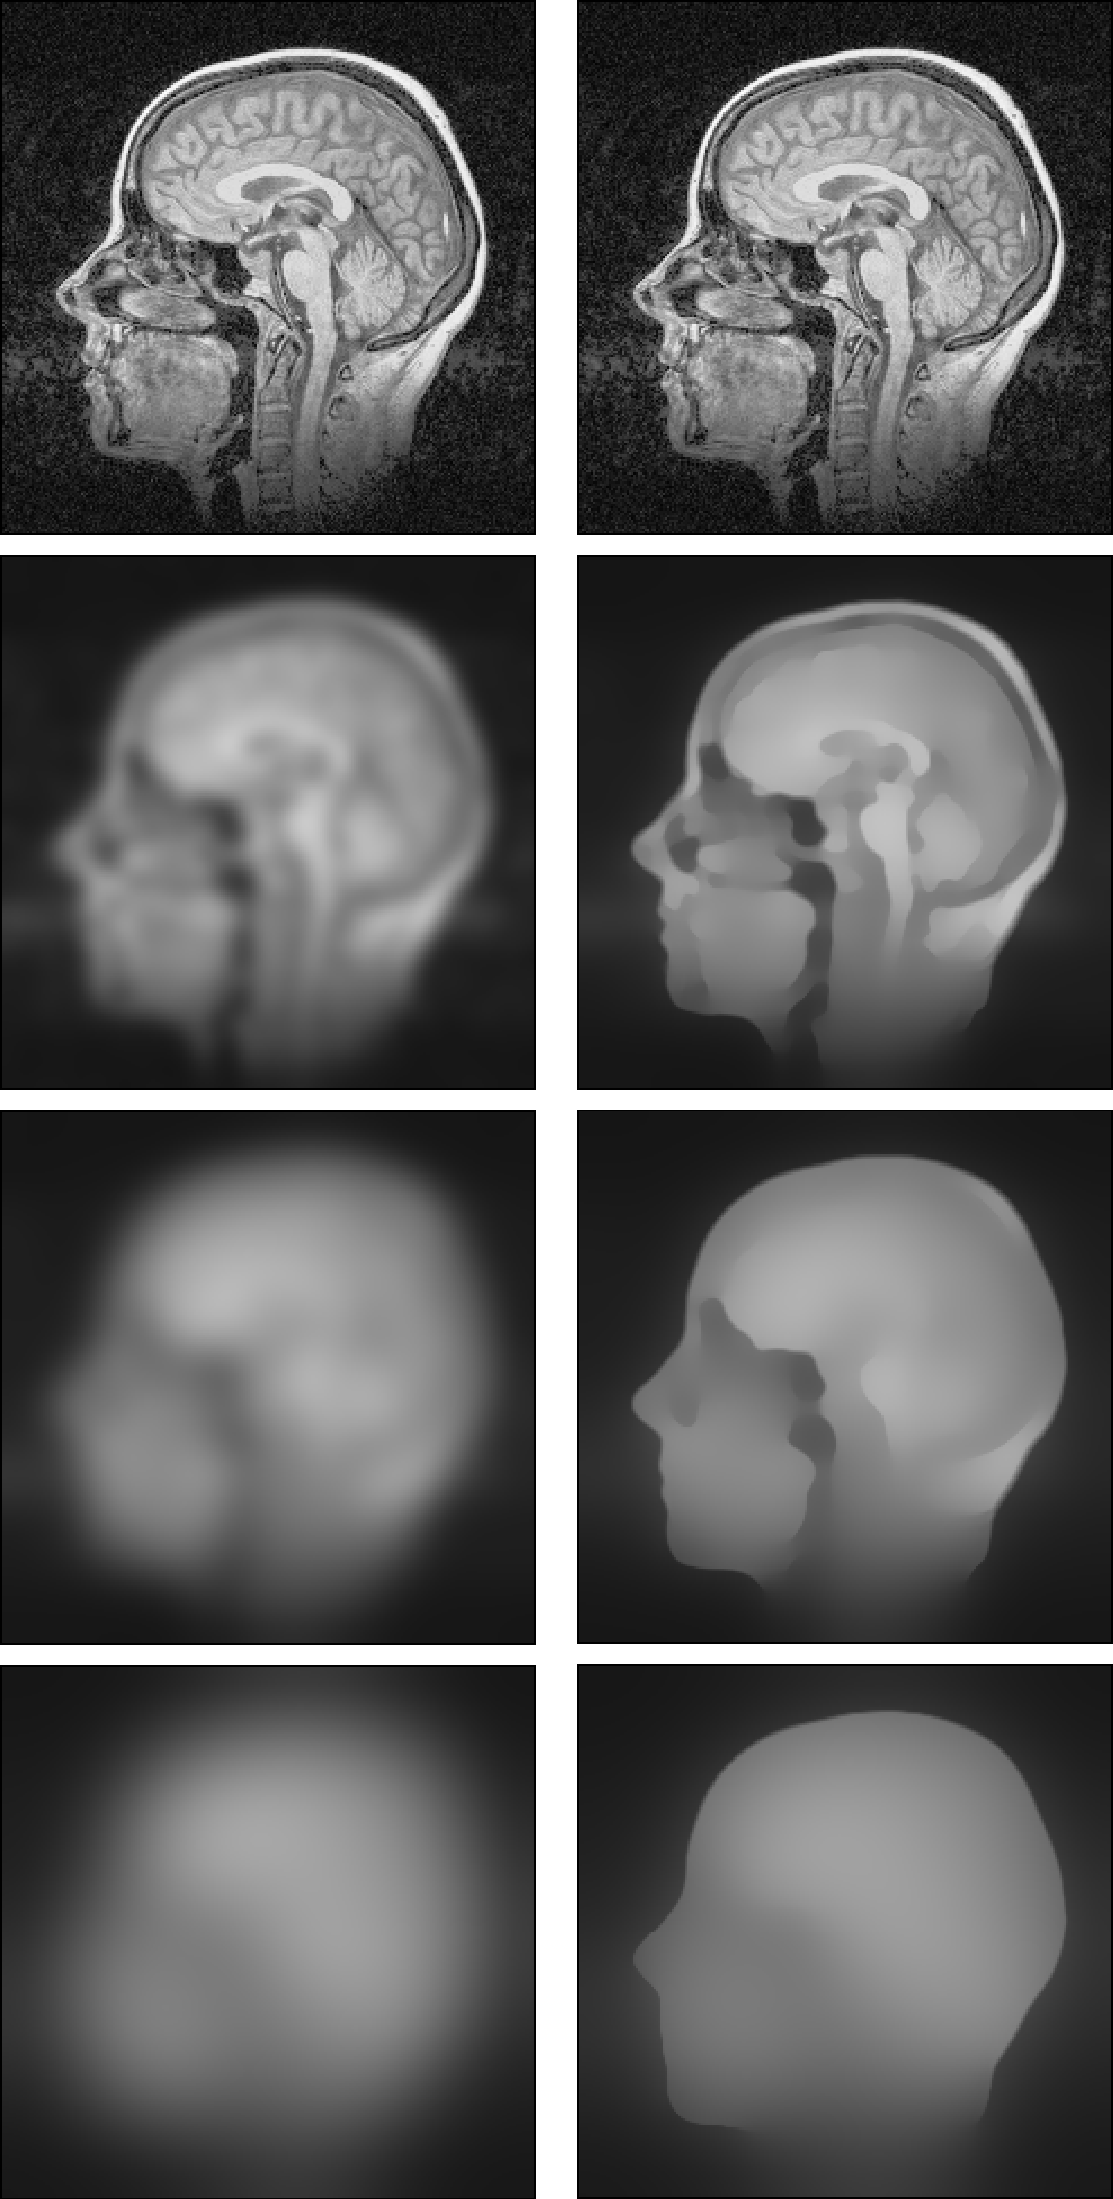
\includegraphics[width=.5\textwidth]{gfx/lin_vs_nonlin_diffusion2.png}
      \caption[Linear vs. nonlinear diffusion]{Image from \citep[p.120,121]{weickert1998}. Linear diffusion on the left,
   anisotropic nonlinear diffusion on the right.}
   \label{fig:lin_vs_nonlin_diffusion}}
\end{figure}

The AKAZE descriptor is obtained from dividing the image region around a
keypoint into a grid and then performing binary tests between all such grid
cells $i,~j$ which test whether $f(i) > f(j)$ for some function $f$ which
encapsulates some information of the cell \citep{yang2012}. To achieve rotation
invariance, this grid is rotated according to the dominant orientation computed
by considering the image derivatives---already computed for the detection---in
the neighbourhood \citep{alcantarilla2012}. The results of these binary tests are
assembled into a binary vector. Its size can be adjusted by making the grid
coarser or finer. For $f$, \citet{alcantarilla2012} consider both intensity
differences and the two image derivatives. The three properties are referred to as
\emph{channels} and the descriptor may include one, two or all three of them,
with three yielding best performance.

\section{Scale Ambiguity}

Computing relative translation between two cameras from corresponding image
points is possible only up to an unknown scale (see
\autoref{sec:eight-point}), meaning it is impossible to determine e.g. if an
object viewed by the camera is small and close or large and further away. That
fact alone would not be problematic, but an iterative procedure requires to
maintain a consistens scale for all estimates of necessary motion.
This poses the problem of how to determine if the user is close to the
desired viewpoint and whether or not they have come closer or moved further
away over the iterations. 

\section{Practical Problems}
\label{sec:app_challenges}

In the context of a rephotography application as in \citep{bae2010}, five
primary obstacles in viewpoint reconstruction of a historic photograph can be
identified.
\begin{enumerate}
   \item The necessary camera motion has six degrees of freedom---three for
      translation and three for rotation---which are challenging for the user
      to adjust simultaneously, as changing one parameter will often necessitate
      adjustments for the others to improve the registration. Furthermore, the
      number of degrees of freedom makes it difficult to communicate to the
      user how they must move the camera.
   \item The estimate for relative translation between two views will be defined
      only up to an unknown scale (see above)
   \item The original photo cannot be used directly for pose retrieval, because
      the estimate degenerates when the user approaches the original viewpoint
      (see above)
   \item Automated computation of relative camera pose will rely on feature
      detection to find correspondences. However, historical images will often
      be vastly different from the current scene. Not only may the scene itself
      have changed considerably, but also the historical image---having been
      taken by a historical camera---may differ in contrast, sharpness and
      colours. Neither SIFT nor AKAZE will reliably find correspondences between
      such an image and a current photo.
   \item The calibration data---most importantly, focal length and principal
      point---of the historical camera are often unknown. The calibration data
      is needed for relative pose computation (see \autoref{sec:epipolar}).
\end{enumerate}

\citet{bae2010} address all these issues in the following way.
Initially, after loading a historical image, the user is instructed to
take two photographs of the scene with a reasonably wide baseline (about
20\textdegree). One of them, termed \emph{first frame} is supposed to be
taken from some distance from the original viewpoint, the \emph{second
frame} should be the user's best eyeballed approximation of it. The wide
baseline allows for a more reliable 3D-reconstrution of the scene used to
tackle problems 2. and 3. 

SIFT features are computed and matched between the two images.  Given these
correspondences, 3D coordinates of the points can be computed. A selection of
these is reprojected into the second frame after which the user identifies six
or more points in the historical photograph corresponding to these points in the
second frame. This allows estimating extrinsic and intrinsic camera parameters
of the historical camera by running an optimisation algorithm on an initial
estimate for relative rotation and translation between first frame and reference
image. Also sensor skew, focal length and principal point of the historical
camera can be inferred this way (problem 5.).  The reference photograph
is not needed anymore after this initial step, circumventing problem 4.  The
principal point's initial guess is found again with help of the user who
identifies three sets of parallel lines in the historical image
\citep[see][chapter 8.8]{h&z2004}.

In this work, this problem is neglected and it is assumed that the original
image can be matched with current photographs, so it should not actually be
historic. This restriction is envisioned to be removed in the future.

A this point the pose of the reference camera relative to the first
camera $T_{\text ref,first},~R_{\text ref,first}$ is known. During the homing
process, the current camera frame is compared to the first frame (not the
reference frame, avoiding problem 3.), which avoids degeneracy due to the wide
baseline. Thus one obtains $T_{\text current,first},~R_{\text current,first}$.
Given the locations of the reference camera and the current frame's camera, each
relative to the first frame, one can compute the location of the reference
relative to the current frame and thus guide the user in the right
direction\footnote{Depending on the coordinate system used and whether $R$ and
   $T$ are given such that they transform points from frame $1$ to frame $2$ or vice
versa, the equations will look different, as they do in \citep{bae2010}}.

\begin{IEEEeqnarray}{rCllt}
   \sub{X}{ref}      & =  & \sub{R}{ref,first}\sub{X}{first} + \sub{T}{ref,first} & \hspace{1em}\\
   \sub{X}{current}  & =  & \sub{R}{current,first}\sub{X}{first} + \sub{T}{current,first}\\[\baselineskip]
   \sub{X}{first}    & =  & \sub{R^T}{current,first}\left(\sub{X}{current} - \sub{T}{current,first}\right) && (1, $R$ orthogonal)\IEEEnonumber\\
   \sub{X}{ref}      & =  & \sub{R}{ref,first}\sub{R^T}{current,first}\left(\sub{X}{current} - \sub{T}{current,first}\right) \\
                     &    & + \sub{T}{ref,first} & & (2, substitute 1)\IEEEnonumber\\
   \sub{X}{ref}      & =  & \sub{R}{ref,first}\sub{R^T}{current,first}\sub{X}{current} \IEEEnonumber\\
                     &    & - \sub{R}{ref,first}\sub{R^T}{current,first}\sub{T}{current,first} + \sub{T}{ref,first}
\end{IEEEeqnarray}
and thus
\begin{equation}\label{eq:necessary_trans}
   \sub{T}{ref,current} = - \sub{R}{ref,first}\sub{R^T}{current,first}\sub{T}{current,first} + \sub{T}{ref,first}
\end{equation}
and
\begin{equation}\label{eq:necessary_rot}
   \sub{R}{ref,current} = \sub{R}{ref,first}\sub{R^T}{current,first}
\end{equation}

During homing, Bae et. al warp the current camera frame according to the
necessary rotation before being shown to the user, allowing them to focus only
on the translation (problem 1.). This is possible since for rephotography
dealing with structures usually at some distance, the rotation will be small,
otherwise the warped image would be unusable. This kind of support is also
disregarded in this work, as achieving the correct rotation with the help of an
overlayed edge image is easy enough, as long as one is directed to the correct
spot. Therefore, only the translation is communicated.

A remaining problem (2.) is that the scale of the necessary translation is
unknown, so that only the direction can be determined. This poses the question
of how to find out whether the user has come closer to the goal or not. It may
be feasible to find the original viewpoint nonetheless, if it could be
determined at least when the user reaches it, but this is not the case without
further information. On top of that, it would make for a better user experience
if also the distance to the goal could be communicated.

A key observation in this regard is that the actual scale of the translation is
irrelevant, it is sufficient that there be a way to make the scale consistent
accross iterations. That is, it is unnecessary to know whether the goal is a
specific distance away, if one can ensure that the translations computed one
after the other can be somehow meaningfully compared. For this, \citet{bae2010}
observe that when triangulating 3D coordinates from corresponding points, their
computed distance from the camera (the first frame) is inversely proportional
to the distance between the cameras. An intuition can be obtained from
\autoref{fig:scale}. To measure the scale of the world, the application uses the
matches between two images and computes 3D coordinates by triangulation. The
average distance of those points to the first frame's camera centre is computed
and compared across iterations to make the scale consistent.

\begin{figure}
   {\centering      
      \begin{subfigure}{\linewidth}
         \begin{tikzpicture}[very thick,node distance=2em]
   \tikzset{>=Latex}
   \def\camAngle{60}
   \def\arrowLength{3em}
   \node[label={180:{$c_1$}}] (c1) at (0,0) {};
   \fill (c1) circle (3pt);
   \node[below left=of c1] {first frame};
   \draw[->] (c1) -- (\camAngle:\arrowLength);
   \node[minimum size=1em,draw,label={90:Object}] (object) at (\camAngle:3cm) {};
   \draw[dashed,name path=line1] (c1) -- (object) node[label={180:{$o_1$}}] {};
   \node[right=3cm of c1,label={0:{$c_2$}}] (c2) {};
   \fill (c2) circle (3pt);
   \draw[->] (c2) -- ($(c2) !3em! (object)$) coordinate (tmp);
   \draw[dashed,name path=line2] (c2) -- (object);
   \node[below right=of c2] {current frame};
   \draw[thin,|-|] ($(c1) + (0,-1em)$) -- ($(c2) + (0,-1em)$) node[below,midway] {$b=1$};

   \draw[thin] (c1) ++(\camAngle:\arrowLength) arc (\camAngle:0:\arrowLength) -- (c1);
   \node at (\camAngle/2:2em) {$\alpha$};

   \pgfmathanglebetweenpoints{\pgfpointanchor{c2}{center}}{\pgfpointanchor{object}{center}}
   \let\reverseAngle\pgfmathresult
   \draw[thin] (tmp) arc (\reverseAngle:180:\arrowLength) -- (c2);
   \pgfmathparse{\reverseAngle+(180-\reverseAngle)/2}
   \node at ($(c2) + (\pgfmathresult:2em)$) {$\beta_1$};

   \coordinate (tmp1) at ($(c1) + (0,1.5cm)$);
   \coordinate (tmp2) at ($(c2) + (0,1.5cm)$);
   \path[name path=second baseline] (tmp1) -- (tmp2);
   \path[name intersections={of=second baseline and line1}] (intersection-1) coordinate (second c1);
   \path[name intersections={of=second baseline and line2}] (intersection-1) coordinate (second c2);
   \fill (second c1) circle (3pt) node[label={180:{$c_1^\prime$}}] {};
   \fill (second c2) circle (3pt) node[label={0:{$c_2^\prime$}}] {};
   \draw[|-|,thin,transform canvas={yshift=-1em}] (second c1) -- (second c2) node[below,midway] {$b^\prime$};

   % \draw[thin,|-|,transform canvas={shift=(90+\camAngle:1em)}] (second c1) -- (object);
\end{tikzpicture}


         \caption{Per the intercept theorem $\frac{|s c_1^\prime|}{|s c_1|} = \frac{b^\prime}{b}$.  
         With increasing baseline, $|s c_1|$ also increases to fulfil the equation.}
      \end{subfigure}

      \begin{subfigure}{\linewidth}
         \begin{tikzpicture}[very thick,node distance=2em]
   \tikzset{>=Latex}
   \def\camAngle{60}
   \def\arrowLength{3em}
   \node[label={180:{$c_1$}}] (c1) at (0,0) {};
   \fill (c1) circle (3pt);
   \node[below left=of c1] {first frame};
   \draw[->] (c1) -- (\camAngle:\arrowLength);
   \node[minimum size=1em,draw] (object) at (\camAngle:3cm) {};
   \draw[dashed,name path=line1] (c1) -- (object) node[label={180:{$o_2$}}] {};
   \node[label={0:{$c_3$}},right=5cm of c1] (c3) {};
   \fill (c3) circle (3pt);
   \draw[->] (c3) -- ($(c3) !3em! (object)$) coordinate (tmp);
   \draw[dashed,name path=line2] (c3) -- (object);
   \node[below right=of c3] {current frame};

   \pgfmathanglebetweenpoints{\pgfpointanchor{c3}{center}}{\pgfpointanchor{object}{center}}
   \let\reverseAngle\pgfmathresult
   \draw[thin] (tmp) arc (\reverseAngle:180:\arrowLength) -- (c3);
   \pgfmathparse{\reverseAngle+(180-\reverseAngle)/2}
   \node at ($(c3) + (\pgfmathresult:2em)$) {$\beta_2$};

   \draw[thin,|-|] ($(c1) + (0,-1em)$) -- ($(c3) + (0,-1em)$) node[below,midway] {$b=1$};

   % \draw[thin,|-|,transform canvas={shift=(90+\camAngle:1em)}] (second c1) -- (object);
\end{tikzpicture}


         \caption{For another baseline, the estimate will still yield a translation
         with unit length.}
      \end{subfigure}

      \begin{subfigure}{\linewidth}
         \begin{tikzpicture}[very thick,node distance=2em]
   \tikzset{>=Latex}
   \def\camAngle{60}
   \def\arrowLength{3em}
   \node[label={180:{$c_1$}}] (c1) at (0,0) {};
   \fill (c1) circle (3pt);
   \node[below left=of c1] {first frame};
   \draw[->] (c1) -- (\camAngle:\arrowLength);
   \node[minimum size=1em,draw] (object) at (\camAngle:3cm) {};
   \draw[dashed,name path=line1] (c1) -- (object) node[label={180:{$s$}}] {};
   \node[label={0:{$c_2$}},right=3cm of c1] (c2) {};
   \fill (c2) circle (3pt);
   \draw[dashed,name path=line2] (c2) -- (object);
   \node[below right=of c2] {current frame};

   \draw[->] (c2) -- ($(c2) !3em! (object)$) coordinate (tmp);


   \draw[thin,|-|] ($(c1) + (0,-1em)$) -- ($(c2) + (0,-1em)$) node[below,midway] {$b=1$};

   % \draw[thin,|-|,transform canvas={shift=(90+\camAngle:1em)}] (second c1) -- (object);

   \begin{scope}[transform canvas={xshift=-2cm}]
      \node[label={180:{$c_3$}},right=5cm of c1] (c3) {};
      \fill (c3) circle (3pt);
      \draw[->] (c3) -- ($(c3) !3em! (object)$) coordinate (tmp);
   \end{scope}
   \coordinate (tmp1) at ($(c3) + (-2cm,0)$);
   \coordinate (tmp2) at ($(tmp) + (-2cm,0)$);
   \path[name path=line3] (tmp1) -- ($(tmp1) !5cm! (tmp2)$);
   \draw[name intersections={of=line1 and line3}]
   node[label={180:{$s_2$}},minimum size=1em,draw,fill=white] (object2) at (intersection-1) {};
   \draw[dashed] (tmp1) -- (object2);
\end{tikzpicture}


         \caption{Equalising the scales in both estimates shows that the distance
         of the object to $c_1$ is smaller if $c_3$ was further away than $c_2$}
      \end{subfigure}

      \caption[Relation between object distance and camera baseline]{The camera
         baseline length is inversely proportional to the distance of the viewed
         object to one of the cameras. Evaluating the distance of viewed objects to
         the first frame's camera yields a measure for how far the two cameras are
      apart.}
   \label{fig:scale}}
\end{figure}

Therefore, in each iteration, the scale of the world is computed by
triangulating correspondences between the first and current frames and computing
the average distance to the first frame's camera. The scale is
compared to the scale computed in the initial step for the first and second
frames. Scaling the current translation vector by the ratio of the
two scales makes the length consistent across iterations and decreasing with the
distance to the goal. However, as this estimate relies on the intercept theorem,
it is only valid as long as the user moves on a straight line between the
initial estimate (position of the second frame) and the goal. Empirical
analysis (see evaluation in \autoref{ch:evaluation}) demonstrates that strong
movement along the optical axis will decrease the usefulness of the scale
estimation. However, in reality this should be a minor problem, as the movement
around a scene will be stronger than towards or away from it when
rephotographing.

For a summary, \autoref{fig:procedure} shows the complete pipeline.
\begin{figure}[h]
   {\centering      
      \begin{tikzpicture}[
      very thick,
      node distance=1.5cm,
      every node/.append style={font=\small,text width=1.5cm,text centered},
      circle node/.style={inner sep=0,shape=circle,draw},
      boxnode/.style={outer sep=0,inner
         sep=4pt,fill=RoyalBlue,text=white,draw=gray,shape=rectangle,rounded
      corners=5pt,minimum height=1.3cm},
      descision node/.style={diamond,aspect=3,inner sep=5pt,draw,text centered},
   ]

   \makegrayinprint

   \tikzset{>=latex}
   \node[boxnode] (ref) {Reference photo};
   \node[boxnode,right=of ref] (first frame) {First frame};
   \node[boxnode,right=of first frame] (second frame) {Second frame};
   \node[draw] (t first ref) at ($(ref) !.5! (first frame) + (0,-3cm)$) {$T_{\text first,ref}$};

   \node[circle node] (triangulation) at ($(first frame) !.5! (second frame) +
   (0,-3cm)$) {Triangu-lation};

   \coordinate (c) at ($(t first ref.north) + (0,1em)$);

   \node[above] at (c) {\texttt{AKAZE}};
   \draw[->] (ref.south) |- (c) -- (t first ref);
   \draw[->] (first frame.south) |- (c) -- (t first ref);
   \draw (first frame) -- coordinate[midway] (c) (second frame);
   \draw[->] (c) -- (triangulation);
   \draw[->] (triangulation) -- (t first ref);
   \node[above] at (c) {\texttt{AKAZE}};

   \begin{scope}[shift={(0cm,-5cm)}]
      \node[opacity=.5,anchor=north west,inner sep=0] at (0,0) {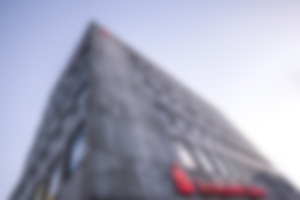
\includegraphics[width=3cm]{gfx/pic.jpg}};
      \draw (0,0) rectangle (3,-2);
      \node (current frame) at (1.5,-0.5) {Current frame};
      \draw[ultra thick,xshift=-1em,->] (1.5,-1.5) -- ++(100:1em);
      \draw[ultra thick,xshift=+1em,->] (1.5,-1.5) -- ++(30:1em);

      \node[circle node,right=of current frame] (triangulation2)
      {Triangu-lation};
      \node[draw,text width={}] (t first current) at ($(current frame) !.5! (triangulation2) +
      (0,-3cm)$) {$T_{\text first,current}$};

      \node[descision node,below=1cm of t first current,inner sep=10pt] (ifequal) {$T_{\text first,current} = T_{\text first,ref}$?};
      \node[boxnode,right=of t first current] (final frame) {Final image};

      \draw[->] (ifequal.west) -- ++(-2cm,0) |- (0,-1) node[midway,left=1em,rotate=90] {No};
      \draw[->] (ifequal.east) -| (final frame.south) node[midway,right=-1em] {Yes};

      \coordinate (c) at ($(t first current.north) + (0,1em)$);
      \draw[->] (c) -- (t first current);
      \draw (triangulation2) |- (c);

      \draw[->] (first frame.north) -- ++(0,1em) -- ++(-5cm,0) -- ++(0,-4cm)
      node[rotate=90,left=1em,midway]
      {\texttt{AKAZE}} |-
      (1.5,1) -| (triangulation2.north);
      \draw[->] (1.5,0) -- ++(0,1);
      \draw (3.5,1) |- (c);
      \draw[->] (t first current) -- (ifequal);

      \draw[|-|] (8.5cm,0) -- ++(0,-6cm) node[right=1em,midway,rotate=90,anchor=center] {Iterate};
   \end{scope}
   \draw[|-|] (8.5cm,1cm) -- ++(0,-4cm) node[right=1em,midway,rotate=90,anchor=center] {Preprocessing};
\end{tikzpicture}

      \caption{Computational rephotography procedure}
   \label{fig:procedure}}
\end{figure}


\chapter{Evaluation}
\label{ch:evaluation}

The approach has been evaluated on two realistic datasets. The most important
questions are whether the direction of the necessary translation is correctly
identified and its scale decreasing with distance to the target.
For both sets of images, the ground-truth translation between each image and the
first frame has been measured with centimetre accuracy, while the ground-truth
rotation has been estimated from manually labelled correspondence as it is
difficult to measure without the proper instruments. Since for the case of
noise-free correspondences in a non-degenerate configuration, relative pose
estimation algorithms are mathematically correct, this has been deemed
sufficiently accurate to evaluate the procedure. For each image pair, 19--27
correspondences have been labelled, of which the majority is used for pose
recovery. For pose recovery, RANSAC is used in conjunction with the five-point
solver, a point is considered an inlier for a given essential matrix if its
distance to its epipolar line is no more than three pixels. These parameters
lead to the majority of points being inliers of the pose recovery, the few
outliers can be explained by imprecise labelling.

In both data sets, the translation was mostly in the horizontal direction and
along the optical axis; the vertical translation is thus neglected. Similarly,
rotation was applied mainly around the vertical axis.

In order to idealise the condition, the reference photograph has been used to
fill the role of the second frame for world scale computation. In reality, since
the reference location is unknown, the reference world scale is obtained from a
position somewhat off.

In all plots $s$ refers to the scale at which the relative pose is computed.
Besides the full resolution, the images are scaled down by factor of $2$ (both
dimensions are halved, resulting in quarter size) and $4$ (sixteenth size). The
resolutions evaluated are thus $3264\times2448$, $1632\times1224$, and
$816\times612$.

The following graphics illustrate three things
\begin{enumerate}
   \item The difference between the computed necessary rotation and the actually
      necessary one
   \item The difference in direction of the computed necessary translation and
      the actually necessary one
   \item The correlation between the true ratio of distances obtained by
      measuring camera movement and the average distance ratio computed with first
      and second (or in this case reference) frames based on automatic feature matching, at
      three different scales
\end{enumerate}

\section{Train Station Data Set}

In this series, the camera was moved horizontally from the reference to the
right while also coming closer to the building.
A schematic bird's eye view of the captures is shown in \autoref{fig:train_scene}.

\begin{figure}[h]
   {\centering      
      \begin{tikzpicture}
   \begin{axis}[
         xmin = -1,
         xmax = 6,
         ymin = -1,
         ymax = 6,
         xlabel = $x$,
         ylabel = $y$,
         every node near coord/.append style={yshift=-0.5cm,anchor=-10} % hacky way putting nodes below points instead of above
      ]
      \addplot+[
         nodes near coords,
         only marks,
         point meta=explicit symbolic,
      ]
      coordinates {
         (0,0)        [0]
         (5.65,2.65)  [1]
         (3.12,0.16)  [2]
         (0.83,0.03)  [3]
         (0.20,0.03)  [4]
         (2,5)        [station]
      };

      \coordinate (station) at (axis cs:2,5);

      \foreach \x / \y in {0/0,5.65/2.65,3.12/0.16,0.83/0.03,0.20/0.03}
      {
         \edef\temp{
            \noexpand\node[outer sep=0,inner sep=0] (foo) at (axis cs:\x,\y) {}; 
         \noexpand\draw[->] (foo) -- ($ (foo) !1cm! (station) $);
      }
         \temp
      }

   \end{axis}
\end{tikzpicture}

      \caption[Schematic of the train scene]{Schematic representation of the Train Station data set. Lengths and angles are not
      precise.}
   \label{fig:train_scene}}
\end{figure}
\autoref{tab:train_data} summarises the ground truth for the five images.

\subsection{Scale Estimation}

\newcolumntype{m}{>{$}c<{$}} % math column
\rowcolors{2}{gray!5}{white} % alternating colours

\begin{table}[h]
   \caption[Train data ground truth]{Ground truth for the train data. Image 0 is the reference frame,
      translations and rotations are given as in \eqref{eq:camera_transform}
   relative to the reference frame.}
   \begin{tabular}{cmmm}
      \toprule
      \rowcolor{white}
      Image        & \text{Relative translation} & \text{Relative Rotation} & \text{ratio}\\
      number       & [x,y,z]                         & [\theta_x, \theta_y, \theta_z]
      \\
      \midrule
      0 & [0      , 0 , 0]      & [0        , 0       , 0]       & 1      \\
      1 & [ .9053 , 0 , .4246 ] & [ -3.3779 , -9.3779 , 1.05121] & 3.8936 \\
      2 & [ .9986 , 0 , .0512 ] & [ -1.3274 , -5.7134 , -.1884 ] & 1.6461 \\
      3 & [ .9993 , 0 , .0361 ] & [ -1.7156 , -2.4761 , .3469  ] & 1.0965 \\
      4 & [ .9950 , 0 , .0995 ] & [ .054606 , -4.4867 , .2452  ] & 1.0343 \\\bottomrule
   \end{tabular}
   \label{tab:train_data}
\end{table}

\autoref{fig:train_dist_ratio} shows how the average distance of points to the
first frame's camera varies with the second image used for triangulation. The
plot illustrates that---especially at full resolution---the ratio based on
feature matching closely mirrors the real value. The difference increases with
decreasing image scale, but the slope of the graphs is quite similar. This
shows that indeed with increasing distance to the first frame, the ratio
decreases, allowing a deduction as to how close the camera is to the target, at
least with respect to previous iterations, which is the primary objective. 
The decrease in ratio closely correlates with the decrease in distance which
is apparent on inspection of \autoref{fig:train_scene}. For instance, the viewpoints
3 and 4 are much closer together than e.g. 2 and 3, and the difference in ratios
is much smaller between 3 and 4 as well. 

The correlation is higher for AKAZE
features than for SIFT ones, where a strong spike for image 1 can be observed.
For SIFT, the decrease of ratio between images 2 and 3 is also hardly visible at
$s=2$. The unusual spike for image 1 poses the problem that the visualisation
would tell the user that they need to move disproportionally far compared to
the other images. Since the error in this case is corrected for the next image,
this may not be a big problem, but will affect user experience. For SIFT
features, one can also observe that the scale of the images appears to be less
relevant, possibly an indication for the better scale invariance of the
descriptor.

Generally, it can be concluded that on this data set, AKAZE features are an
appropriate means of estimating the scale of relative camera translation.

\begin{figure}[h]
   \begin{subfigure}{.5\linewidth}
      \centering      
      \pgfplotstableread[col sep=space]{data/bahnhof_detector_KAZE_resize_1_ratio_0.800000.dat}\datatablenoresize
\pgfplotstableread[col sep=space]{data/bahnhof_detector_KAZE_resize_2_ratio_0.800000.dat}\datatableresize
\pgfplotstableread[col sep=space]{data/bahnhof_detector_KAZE_resize_4_ratio_0.800000.dat}\datatabledoubleresize
\begin{tikzpicture}
   \begin{axis}[
         xlabel={Image Number},
         ylabel={Distance ratio},
         ymax=4.5,
         xtick=data,
         % xticklabels from table={\datatable}{fname}
         scale=.6, % dare you to change this to sth larger
         legend pos=north east,
      ]

      % original size
      \addplot table[
         x expr=\coordindex,
         y=realdist_ratio,
      ] {\datatablenoresize};
      \addlegendentry{Truth}

      \addplot table[
         x expr=\coordindex,
         y=dist_ratio,
      ] {\datatablenoresize};
      \addlegendentry{$s=1$}

      % scaled by 2
      \addplot table[
         x expr=\coordindex,
         y=dist_ratio,
      ] {\datatableresize};
      \addlegendentry{$s=2$}

      % scaled by 2
      \addplot table[
         x expr=\coordindex,
         y=dist_ratio,
      ] {\datatabledoubleresize};
      \addlegendentry{$s=4$}

   \end{axis}
\end{tikzpicture}

      \caption{AKAZE features}
      \label{fig:train_KAZE_dist_ratio}
   \end{subfigure}
   \quad
   \begin{subfigure}{.5\linewidth}
      \centering      
      \pgfplotstableread[col sep=space]{data/bahnhof_detector_SIFT_resize_1_ratio_0.800000.dat}\datatablenoresize
\pgfplotstableread[col sep=space]{data/bahnhof_detector_SIFT_resize_2_ratio_0.800000.dat}\datatableresize
\pgfplotstableread[col sep=space]{data/bahnhof_detector_SIFT_resize_4_ratio_0.800000.dat}\datatabledoubleresize
\begin{tikzpicture}
   \begin{axis}[
         xlabel=\vphantom{Image Number},
         % ylabel={Distance ratio},
         % ymax=11, % changing this to 10 will fuck up the subfigure. dafug.
         yticklabel pos=right,
         xtick=data,
         ymode=log,
         % xticklabels from table={\datatable}{fname},
         legend pos=north east,
         scale=.6,
      ]

      % original size
      \addplot table[
         x expr=\coordindex,
         y=realdist_ratio,
      ] {\datatablenoresize};
      \addlegendentry{Ground truth}

      \addplot+[dashed,mark=o] table[
         x expr=\coordindex,
         y=dist_ratio,
      ] {\datatablenoresize};
      \addlegendentry{$s=1$}

      % scaled by 2
      \addplot+[dashed,mark=o] table[
         x expr=\coordindex,
         y=dist_ratio,
      ] {\datatableresize};
      \addlegendentry{$s=2$}

      % scaled by 4
      \addplot+[dashed,mark=o] table[
         x expr=\coordindex,
         y=dist_ratio,
      ] {\datatabledoubleresize};
      \addlegendentry{$s=4$}

   \end{axis}
\end{tikzpicture}




      \caption{SIFT features}
      \label{fig:train_SIFT_dist_ratio}
   \end{subfigure}
   \caption[Train data: Distance ratio]{Train Station data set: Evolution of the distance ratio between images}
   \label{fig:train_dist_ratio}
\end{figure}

\subsection{Rotation Estimation}

\autoref{fig:train_rotation_KAZE} and \autoref{fig:train_rotation_SIFT} illustrate the
difference between the actually necessary camera rotation and the computed one
for AKAZE and SIFT features, respectively. Rotations about the optical an X axes
are small and thus not very interesting and the deviation is small. 

Focusing on the Y-rotation, it is obvious is that the estimation
quality decreases especially for $s=4$, but the difference does not exceed 5
degrees and thus the estimate is very usable, especially since for reasonably
quick updates, mostly the direction of necessary rotation is important, not the
absolute magnitude.

The performance of SIFT is even better for scales $s=1$ and $s=2$, but slightly
worse on the smallest scale (see \autoref{fig:train_SIFT_rotation_4}).

\begin{figure}[h]
   \begin{subfigure}{.5\linewidth}
      \centering      
      \pgfplotstableread[col sep=space]{data/bahnhof_detector_KAZE_resize_1_ratio_0.800000.dat}\datatable
\begin{tikzpicture}
   \begin{axis}[
         xlabel={Image Number},
         ylabel={Rotation angles},
         xtick=data,
         cycle list name=mylist,
         scale=.7,
      ]

      % original size
      \addplot table[
         x expr=\coordindex,
         y=realthetax,
      ] {\datatable};
      \addlegendentry{True $\theta_x$}
      \addplot table[
         x expr=\coordindex,
         y=realthetay,
      ] {\datatable};
      \addlegendentry{True $\theta_y$}
      \addplot table[
         x expr=\coordindex,
         y=realthetaz,
      ] {\datatable};
      \addlegendentry{True $\theta_z$}

      % half size
      \addplot table[
         x expr=\coordindex,
         y=thetax,
      ] {\datatable};
      \addlegendentry{$\theta_x$}
      \addplot table[
         x expr=\coordindex,
         y=thetay,
      ] {\datatable};
      \addlegendentry{$\theta_y$}
      \addplot table[
         x expr=\coordindex,
         y=thetaz,
      ] {\datatable};
      \addlegendentry{$\theta_z$}

   \end{axis}
\end{tikzpicture}



      \caption{$s=1$}
      \label{fig:train_KAZE_rotation_1}
   \end{subfigure}
   \quad
   \begin{subfigure}{.5\linewidth}
      \centering      
      \pgfplotstableread[col sep=space]{data/bahnhof_detector_KAZE_resize_2_ratio_0.800000.dat}\datatable
\begin{tikzpicture}
   \begin{axis}[
         xlabel={\vphantom{Image Number}},
         xtick=data,
         cycle list name=mylist,
         scale=.7,
         yticklabels={},
      ]

      % original size
      \addplot table[
         x expr=\coordindex,
         y=realthetax,
      ] {\datatable};
      \addlegendentry{True $\theta_x$}
      \addplot table[
         x expr=\coordindex,
         y=realthetay,
      ] {\datatable};
      \addlegendentry{True $\theta_y$}
      \addplot table[
         x expr=\coordindex,
         y=realthetaz,
      ] {\datatable};
      \addlegendentry{True $\theta_z$}

      % half size
      \addplot table[
         x expr=\coordindex,
         y=thetax,
      ] {\datatable};
      \addlegendentry{$\theta_x$}
      \addplot table[
         x expr=\coordindex,
         y=thetay,
      ] {\datatable};
      \addlegendentry{$\theta_y$}
      \addplot table[
         x expr=\coordindex,
         y=thetaz,
      ] {\datatable};
      \addlegendentry{$\theta_z$}

   \end{axis}
\end{tikzpicture}




      \caption{$s=2$}
      \label{fig:train_KAZE_rotation_2}
   \end{subfigure}\\[3ex]
   \begin{subfigure}{\linewidth}
      \centering      
      \pgfplotstableread[col sep=space]{data/bahnhof_detector_KAZE_resize_4_ratio_0.800000.dat}\datatable
\begin{tikzpicture}
   \begin{axis}[
         scale=.7,
         cycle list name=mylist,
         xtick=data,
      ]

      % original size
      \addplot table[
         x expr=\coordindex,
         y=realthetax,
      ] {\datatable};
      \addlegendentry{True $\theta_x$}
      \addplot table[
         x expr=\coordindex,
         y=realthetay,
      ] {\datatable};
      \addlegendentry{True $\theta_y$}
      \addplot table[
         x expr=\coordindex,
         y=realthetaz,
      ] {\datatable};
      \addlegendentry{True $\theta_z$}

      % half size
      \addplot table[
         x expr=\coordindex,
         y=thetax,
      ] {\datatable};
      \addlegendentry{$\theta_x$}
      \addplot table[
         x expr=\coordindex,
         y=thetay,
      ] {\datatable};
      \addlegendentry{$\theta_y$}
      \addplot table[
         x expr=\coordindex,
         y=thetaz,
      ] {\datatable};
      \addlegendentry{$\theta_z$}

   \end{axis}
\end{tikzpicture}





      \caption{$s=4$}
      \label{fig:train_KAZE_rotation_4}
   \end{subfigure}
   \caption[Train data: Rotation AKAZE]{Train Station data set: Angles of rotation relative to reference with
   AKAZE features on full, quater and sixteenth resolution}
   \label{fig:train_rotation_KAZE}
\end{figure}

\begin{figure}[h]
   \begin{subfigure}{.5\linewidth}
      \centering      
      \pgfplotstableread[col sep=space]{data/bahnhof_detector_SIFT_resize_1_ratio_0.800000.dat}\datatable
\begin{tikzpicture}
   \begin{axis}[
         xlabel={Image Number},
         ylabel={Rotation angles},
         xtick=data,
         cycle list name=mylist,
         scale=.7,
      ]

      % original size
      \addplot table[
         x expr=\coordindex,
         y=realthetax,
      ] {\datatable};
      \addlegendentry{True $\theta_x$}
      \addplot table[
         x expr=\coordindex,
         y=realthetay,
      ] {\datatable};
      \addlegendentry{True $\theta_y$}
      \addplot table[
         x expr=\coordindex,
         y=realthetaz,
      ] {\datatable};
      \addlegendentry{True $\theta_z$}

      % half size
      \addplot table[
         x expr=\coordindex,
         y=thetax,
      ] {\datatable};
      \addlegendentry{$\theta_x$}
      \addplot table[
         x expr=\coordindex,
         y=thetay,
      ] {\datatable};
      \addlegendentry{$\theta_y$}
      \addplot table[
         x expr=\coordindex,
         y=thetaz,
      ] {\datatable};
      \addlegendentry{$\theta_z$}

   \end{axis}
\end{tikzpicture}



      \caption{$s=1$}
      \label{fig:train_SIFT_rotation_1}
   \end{subfigure}
   \quad
   \begin{subfigure}{.5\linewidth}
      \centering      
      \pgfplotstableread[col sep=space]{data/bahnhof_detector_SIFT_resize_2_ratio_0.800000.dat}\datatable
\begin{tikzpicture}
   \begin{axis}[
         xlabel={\vphantom{Image Number}},
         xtick=data,
         cycle list name=mylist,
         scale=.7,
         yticklabels={},
         legend pos=south east,
         ymin=-10,
         ymax=1,
      ]

      % original size
      \addplot table[
         x expr=\coordindex,
         y=realthetax,
      ] {\datatable};
      \addlegendentry{True $\theta_x$}
      \addplot table[
         x expr=\coordindex,
         y=realthetay,
      ] {\datatable};
      \addlegendentry{True $\theta_y$}
      \addplot table[
         x expr=\coordindex,
         y=realthetaz,
      ] {\datatable};
      \addlegendentry{True $\theta_z$}

      % half size
      \addplot table[
         x expr=\coordindex,
         y=thetax,
      ] {\datatable};
      \addlegendentry{$\theta_x$}
      \addplot table[
         x expr=\coordindex,
         y=thetay,
      ] {\datatable};
      \addlegendentry{$\theta_y$}
      \addplot table[
         x expr=\coordindex,
         y=thetaz,
      ] {\datatable};
      \addlegendentry{$\theta_z$}

   \end{axis}
\end{tikzpicture}




      \caption{$s=2$}
      \label{fig:train_SIFT_rotation_2}
   \end{subfigure}\\[3ex]
   \begin{subfigure}{\linewidth}
      \centering      
      \pgfplotstableread[col sep=space]{data/bahnhof_detector_SIFT_resize_4_ratio_0.800000.dat}\datatable
\begin{tikzpicture}
   \begin{axis}[
         scale=.7,
         cycle list name=mylist,
         xtick=data,
      ]

      % original size
      \addplot table[
         x expr=\coordindex,
         y=realthetax,
      ] {\datatable};
      \addlegendentry{True $\theta_x$}
      \addplot table[
         x expr=\coordindex,
         y=realthetay,
      ] {\datatable};
      \addlegendentry{True $\theta_y$}
      \addplot table[
         x expr=\coordindex,
         y=realthetaz,
      ] {\datatable};
      \addlegendentry{True $\theta_z$}

      % half size
      \addplot table[
         x expr=\coordindex,
         y=thetax,
      ] {\datatable};
      \addlegendentry{$\theta_x$}
      \addplot table[
         x expr=\coordindex,
         y=thetay,
      ] {\datatable};
      \addlegendentry{$\theta_y$}
      \addplot table[
         x expr=\coordindex,
         y=thetaz,
      ] {\datatable};
      \addlegendentry{$\theta_z$}

   \end{axis}
\end{tikzpicture}





      \caption{$s=4$}
      \label{fig:train_SIFT_rotation_4}
   \end{subfigure}
   \caption[Train data: Rotation SIFT]{Train Station data set: Angles of rotation relative to reference with SIFT features}
   \label{fig:train_rotation_SIFT}
\end{figure}

\subsection{Translation Estimation}

Finally and most importantly, the directions of the necessary translation must
be evaluated. \autoref{fig:train_direction} plots the angular difference in
degree between the actual necessary translation and the computed one. The
reference frame $0$ is omitted since the translation vector to compare with is
$(0,0,0)$.

\begin{figure}[h]
   \begin{subfigure}{.5\linewidth}
      \centering      
      \pgfplotstableread[col sep=space]{data/bahnhof_detector_KAZE_resize_1_ratio_0.800000.dat}\datatablenoresize
\pgfplotstableread[col sep=space]{data/bahnhof_detector_KAZE_resize_2_ratio_0.800000.dat}\datatableresize
\pgfplotstableread[col
sep=space]{data/bahnhof_detector_KAZE_resize_4_ratio_0.800000.dat}\datatabledoubleresize
\begin{tikzpicture}
   \begin{axis}[
         xlabel={Image Number},
         ylabel={Angular difference},
         xtick=data,
         legend pos=north east,
         scale=.6,
      ]
      \pgfplotstablegetrowsof{\datatablenoresize}
      \pgfmathsetmacro\yfin{\pgfmathresult - 4}
      \pgfmathsetmacro\yini{0}


      % original size
      \addplot table[
         skip coords between index={\yini}{\yfin},
         x expr=\coordindex,
         y expr={
            acos(
            (
            \thisrow{x}*\thisrow{realx} +
            \thisrow{y}*\thisrow{realy} +
            \thisrow{z}*\thisrow{realz}
            ) / 
            (
            sqrt(
            (\thisrow{x})^2 +
            (\thisrow{y})^2 +
            (\thisrow{z})^2
            ) * 
            sqrt(
            (\thisrow{realx})^2 +
            (\thisrow{realy})^2 +
            (\thisrow{realz})^2
            )
            )
            )
         }
      ] {\datatablenoresize};
      \addlegendentry{$s=1$}

      % quarter size
      \addplot table[
         skip coords between index={\yini}{\yfin},
         x expr=\coordindex,
         y expr={
            acos(
            (
            \thisrow{x}*\thisrow{realx} +
            \thisrow{y}*\thisrow{realy} +
            \thisrow{z}*\thisrow{realz}
            ) / 
            (
            sqrt(
            (\thisrow{x})^2 +
            (\thisrow{y})^2 +
            (\thisrow{z})^2
            ) * 
            sqrt(
            (\thisrow{realx})^2 +
            (\thisrow{realy})^2 +
            (\thisrow{realz})^2
            )
            )
            )
         }
      ] {\datatableresize};
      \addlegendentry{$s=2$}

      % sixteenth size
      \addplot table[
         skip coords between index={\yini}{\yfin},
         x expr=\coordindex,
         y expr={
            acos(
            (
            \thisrow{x}*\thisrow{realx} +
            \thisrow{y}*\thisrow{realy} +
            \thisrow{z}*\thisrow{realz}
            ) / 
            (
            sqrt(
            (\thisrow{x})^2 +
            (\thisrow{y})^2 +
            (\thisrow{z})^2
            ) * 
            sqrt(
            (\thisrow{realx})^2 +
            (\thisrow{realy})^2 +
            (\thisrow{realz})^2
            )
            )
            )
         }
      ] {\datatabledoubleresize};
      \addlegendentry{$s=4$}
   \end{axis}
\end{tikzpicture}

      \caption{AKAZE features}
      \label{fig:train_KAZE_direction}
   \end{subfigure}
   \begin{subfigure}{.5\linewidth}
      \centering      
      \pgfplotstableread[col sep=space]{data/bahnhof_detector_SIFT_resize_1_ratio_0.800000.dat}\datatablenoresize
\pgfplotstableread[col sep=space]{data/bahnhof_detector_SIFT_resize_2_ratio_0.800000.dat}\datatableresize
\pgfplotstableread[col
sep=space]{data/bahnhof_detector_SIFT_resize_4_ratio_0.800000.dat}\datatabledoubleresize
\begin{tikzpicture}
   \begin{axis}[
         xlabel=\vphantom{Image Number},
         % ylabel={Angular difference},
         yticklabels={},
         xtick=data,
         legend pos=north east,
         scale=.6,
         ymin=80,
         ymax=120,
      ]
      \pgfplotstablegetrowsof{\datatablenoresize}
      \pgfmathsetmacro\yfin{\pgfmathresult - 4}
      \pgfmathsetmacro\yini{0}


      % original size
      \addplot table[
         skip coords between index={\yini}{\yfin},
         x expr=\coordindex,
         y expr={
            acos(
            (
            \thisrow{x}*\thisrow{realx} +
            \thisrow{y}*\thisrow{realy} +
            \thisrow{z}*\thisrow{realz}
            ) / 
            (
            sqrt(
            (\thisrow{x})^2 +
            (\thisrow{y})^2 +
            (\thisrow{z})^2
            ) * 
            sqrt(
            (\thisrow{realx})^2 +
            (\thisrow{realy})^2 +
            (\thisrow{realz})^2
            )
            )
            )
         }
      ] {\datatablenoresize};
      \addlegendentry{$s=1$}

      % quarter size
      \addplot table[
         skip coords between index={\yini}{\yfin},
         x expr=\coordindex,
         y expr={
            acos(
            (
            \thisrow{x}*\thisrow{realx} +
            \thisrow{y}*\thisrow{realy} +
            \thisrow{z}*\thisrow{realz}
            ) / 
            (
            sqrt(
            (\thisrow{x})^2 +
            (\thisrow{y})^2 +
            (\thisrow{z})^2
            ) * 
            sqrt(
            (\thisrow{realx})^2 +
            (\thisrow{realy})^2 +
            (\thisrow{realz})^2
            )
            )
            )
         }
      ] {\datatableresize};
      \addlegendentry{$s=2$}

      % sixteenth size
      \addplot table[
         skip coords between index={\yini}{\yfin},
         x expr=\coordindex,
         y expr={
            acos(
            (
            \thisrow{x}*\thisrow{realx} +
            \thisrow{y}*\thisrow{realy} +
            \thisrow{z}*\thisrow{realz}
            ) / 
            (
            sqrt(
            (\thisrow{x})^2 +
            (\thisrow{y})^2 +
            (\thisrow{z})^2
            ) * 
            sqrt(
            (\thisrow{realx})^2 +
            (\thisrow{realy})^2 +
            (\thisrow{realz})^2
            )
            )
            )
         }
      ] {\datatabledoubleresize};
      \addlegendentry{$s=4$}
   \end{axis}
\end{tikzpicture}


      \caption{SIFT features}
      \label{fig:train_SIFT_direction}
   \end{subfigure}
   \caption[Train data: Translation]{Train Station data set: Angular difference between actually necessary translation and algorithmic estimate}
   \label{fig:train_direction}
\end{figure}

It is obvious that the estimates are completely useless, the difference
exceeds $80$ degrees in all cases. The results are so staggeringly bad as to be
suggestive of conceptual or mathematical error, though none could be found. With
these estimates, the user will be sent into an entirely wrong direction.

\FloatBarrier

\section{Manor Data Set}

Seven images (including the reference photo) have been taken with movement to
the right and backwards as well as forwards. The motif was always centred in the
frame, thus there is prominent rotation around the $y$-Axis. 
The schematic positions for the seven manor captures (including reference
photograph) are shown in \autoref{fig:manor_scene}. In contrast to the
train station set, there is more significant movement along the optical axis.

The ground truth data is summarised in \autoref{tab:manor_data}.

\begin{figure}[h]
   {\centering      
      \begin{tikzpicture}
   \begin{axis}[
         xmin = -2,
         xmax = 20,
         ymin = -10,
         ymax = 16,
         xlabel = $x$,
         ylabel = $y$,
         every node near coord/.append style={anchor=5} % hacky way putting nodes below points instead of above
      ]
      \addplot+[
         nodes near coords,
         only marks,
         point meta=explicit symbolic,
         mark=*,
         black,
      ]
      coordinates {
         (0,0)   [0]
         (2,0)   [1]
         (4,2)   [2]
         (4,4)   [3]
         (8,-5)  [4]
         (10,4)  [5]
         (16,-6) [6]
         (16,2)  [first frame]
         (10,15) [manor]
      };

      \coordinate (manor) at (axis cs:10,15);

      \foreach \x / \y in {0/0,2/0,4/2,4/4,8/-5,10/4,16/-6,16/2}
      {
         \edef\temp{
            \noexpand\node[outer sep=0,inner sep=0] (foo) at (axis cs:\x,\y) {}; 
            \noexpand\draw[->] (foo) -- ($ (foo) !.5cm! (manor) $);
         }
         \temp
      }

   \end{axis}
\end{tikzpicture}

      \caption[Schematic of the manor data set]{Schematic representation of the Manor data set. Lengths and angles are not
      precise.}
   \label{fig:manor_scene}}
\end{figure}


\begin{table}[h]
   \caption[Manor data ground truth]{Ground truth for the manor data. Image $0$ is the reference frame,
      translations and rotations are given as in \eqref{eq:camera_transform}
   relative to the reference frame.}
   \begin{tabular}{cmmm}
      \toprule
      \rowcolor{white}
      Image        & \text{Relative translation} & \text{Relative Rotation} & \text{ratio}\\
      number       & [x,y,z]                         & [\theta_x, \theta_y, \theta_z]
      \\
      \midrule
      0 & [0       , 0  , 0]        & [0 , 0        , 0]                & 1       \\
      1 & [ 1      , 0  , 0       ] & [ -1.7857   , -5.4827  , 2.1073 ] & 1.1401  \\
      2 & [ 0.8944 , 0. , 0.4472  ] & [ -2.1428   , -6.5773  , 1.6584 ] & 1.3437  \\
      3 & [ 0.7071 , 0. , 0.7071  ] & [ 0.7263    , -5.0686  , 2.6176 ] & 1.3254  \\
      4 & [ 0.8479 , 0. , -0.5299 ] & [ -1.4146   , -10.7998 , 2.2250 ] & 1.5168  \\
      5 & [ 0.9284 , 0. , 0.3713  ] & [ -0.1887   , -16.6670 , 1.2211 ] & 2.5495  \\
      6 & [ 0.9363 , 0. , -0.3511 ] & [ -0.8725   , -18.0933 , 1.5385 ] & 2.0155  \\\bottomrule
   \end{tabular}
   \label{tab:manor_data}
\end{table}

\subsection{Scale Estimation}

The evolution of the translation scale is shown in \autoref{fig:manor_dist_ratio}.
It is apparent that the movement purely along the optical axis between images
$2$ and $3$ is a problem. As the real distance to the target marginally
increases, so should the ratio, but it decreases instead. Frames $5$ and $6$
illustrate a problem with the scale estimation procedure itself. For it to work
precisely, only movement along the line between first and reference frames is
assumed, as a decreased distance to the first frame is interpreted as an
increased distance to the reference frame, which is not necessarily the case as
shown here. Even the ``ground truth'' computed from actual camera distances is thus
of limited use.

For the AKAZE descriptor, only the full resolution comes reasonably close in
magnitude and somewhat in slope. Wit SIFT, the slope is more accurately
reproduced with $s=2$, but strangely less accurately on full resolution. For the
smallest scale, the estimate degenerates
strongly.

Generally is can be stated that the estimates are less close than those for the
train data set, but also that large movement along the optical axis shows the
limits of this simple approach at scale estimation. Realistically, the user will
not move as erratically so this kind of scenario is extreme.

\begin{figure}[h]
   \begin{subfigure}{.5\linewidth}
      \centering      
      \pgfplotstableread[col sep=space]{data/gut_rosenkrantz_detector_KAZE_resize_1_ratio_0.800000.dat}\datatablenoresize
\pgfplotstableread[col sep=space]{data/gut_rosenkrantz_detector_KAZE_resize_2_ratio_0.800000.dat}\datatableresize
\pgfplotstableread[col sep=space]{data/gut_rosenkrantz_detector_KAZE_resize_4_ratio_0.800000.dat}\datatabledoubleresize
\begin{tikzpicture}
   \begin{axis}[
         xlabel={Image Number},
         ylabel={Distance ratio},
         % xtick=data,
         % xticklabels from table={\datatable}{fname},
         legend pos=north west,
      ]

      % original size
      \addplot table[
         x expr=\coordindex,
         y=realdist_ratio,
      ] {\datatablenoresize};
      \addlegendentry{Ground truth}

      \addplot table[
         x expr=\coordindex,
         y=dist_ratio,
      ] {\datatablenoresize};
      \addlegendentry{$s=1$}

      % scaled by 2
      \addplot table[
         x expr=\coordindex,
         y=dist_ratio,
      ] {\datatableresize};
      \addlegendentry{$s=2$}

      % scaled by 4
      \addplot table[
         x expr=\coordindex,
         y=dist_ratio,
      ] {\datatabledoubleresize};
      \addlegendentry{$s=4$}

   \end{axis}
\end{tikzpicture}


      \caption{AKAZE features}
      \label{fig:manor_KAZE_dist_ratio}
   \end{subfigure}
   \quad\begin{subfigure}{.5\linewidth}
      \centering      
      \pgfplotstableread[col sep=space]{data/gut_rosenkrantz_detector_SIFT_resize_1_ratio_0.800000.dat}\datatablenoresize
\pgfplotstableread[col sep=space]{data/gut_rosenkrantz_detector_SIFT_resize_2_ratio_0.800000.dat}\datatableresize
\pgfplotstableread[col sep=space]{data/gut_rosenkrantz_detector_SIFT_resize_4_ratio_0.800000.dat}\datatabledoubleresize
\begin{tikzpicture}
   \begin{axis}[
         xlabel=\vphantom{Image Number},
         yticklabels={},
         ymin=-0.5,
         ymax=7,
         xtick=data,
         legend pos=north west,
         scale=.7,
      ]

      % original size
      \addplot table[
         x expr=\coordindex,
         y=realdist_ratio,
      ] {\datatablenoresize};
      \addlegendentry{Truth}

      \addplot table[
         x expr=\coordindex,
         y=dist_ratio,
      ] {\datatablenoresize};
      \addlegendentry{$s=1$}

      % scaled by 2
      \addplot table[
         x expr=\coordindex,
         y=dist_ratio,
      ] {\datatableresize};
      \addlegendentry{$s=2$}

      % scaled by 4
      \addplot table[
         x expr=\coordindex,
         y=dist_ratio,
      ] {\datatabledoubleresize};
      \addlegendentry{$s=4$}

   \end{axis}
\end{tikzpicture}



      \caption{SIFT features}
      \label{fig:manor_SIFT_dist_ratio}
   \end{subfigure}
   \caption[Manor Data: distance ratio]{Manor data set: Evolution of the distance ratio between images}
   \label{fig:manor_dist_ratio}
\end{figure}

\subsection{Rotation Estimation}

\autoref{fig:manor_KAZE_rotation} and \autoref{fig:manor_SIFT_rotation}
illustrate how accurately the necessary rotation is computed. On this data, AKAZE
outperforms SIFT with default parameters (see \autoref{sec:something}). On both full and
half scale, there is negligible deviation from the truth, but on quarter scale,
there are more than $5$ degrees of difference and a complete failure for frame
$3$ (the direction is wrong, not only the magnitude).

With default parameters, SIFT compares much worse, particularly on full
resolution where it grossly overestimates the necessary rotation. The results
are better on the scaled-down images, possibly because of the reduction of
noise, but still only partly useful on the smallest resolution.

\begin{figure}[h]
   \begin{subfigure}{.5\linewidth}
      \centering      
      \pgfplotstableread[col sep=space]{data/gut_rosenkrantz_detector_KAZE_resize_1_ratio_0.800000.dat}\datatable
\begin{tikzpicture}
   \begin{axis}[
         xlabel={Image Number},
         ylabel={Rotation angles},
         xtick=data,
         cycle list name=mylist,
         scale=.7,
      ]

      % original size
      \addplot table[
         x expr=\coordindex,
         y=realthetax,
      ] {\datatable};
      \addlegendentry{True $\theta_x$}
      \addplot table[
         x expr=\coordindex,
         y=realthetay,
      ] {\datatable};
      \addlegendentry{True $\theta_y$}
      \addplot table[
         x expr=\coordindex,
         y=realthetaz,
      ] {\datatable};
      \addlegendentry{True $\theta_z$}

      % half size
      \addplot table[
         x expr=\coordindex,
         y=thetax,
      ] {\datatable};
      \addlegendentry{$\theta_x$}
      \addplot table[
         x expr=\coordindex,
         y=thetay,
      ] {\datatable};
      \addlegendentry{$\theta_y$}
      \addplot table[
         x expr=\coordindex,
         y=thetaz,
      ] {\datatable};
      \addlegendentry{$\theta_z$}

   \end{axis}
\end{tikzpicture}



      \label{fig:manor_KAZE_rotation_1}
      \caption{$s=1$}
   \end{subfigure}
   \quad
   \begin{subfigure}{.5\linewidth}
      \centering      
      \pgfplotstableread[col sep=space]{data/gut_rosenkrantz_detector_KAZE_resize_2_ratio_0.800000.dat}\datatable
\begin{tikzpicture}
   \begin{axis}[
         xlabel={\vphantom{Image Number}},
         xtick=data,
         cycle list name=mylist,
         scale=.7,
         yticklabels={},
         ymin=-20,
         ymax=5,
      ]

      % original size
      \addplot table[
         x expr=\coordindex,
         y=realthetax,
      ] {\datatable};
      \addlegendentry{True $\theta_x$}
      \addplot table[
         x expr=\coordindex,
         y=realthetay,
      ] {\datatable};
      \addlegendentry{True $\theta_y$}
      \addplot table[
         x expr=\coordindex,
         y=realthetaz,
      ] {\datatable};
      \addlegendentry{True $\theta_z$}

      % half size
      \addplot table[
         x expr=\coordindex,
         y=thetax,
      ] {\datatable};
      \addlegendentry{$\theta_x$}
      \addplot table[
         x expr=\coordindex,
         y=thetay,
      ] {\datatable};
      \addlegendentry{$\theta_y$}
      \addplot table[
         x expr=\coordindex,
         y=thetaz,
      ] {\datatable};
      \addlegendentry{$\theta_z$}

   \end{axis}
\end{tikzpicture}




      \label{fig:manor_KAZE_rotation_2}
      \caption{$s=2$}
   \end{subfigure}\\[3ex]
   \begin{subfigure}{\linewidth}
      \centering      
      \pgfplotstableread[col sep=space]{data/gut_rosenkrantz_detector_KAZE_resize_4_ratio_0.800000.dat}\datatable
\begin{tikzpicture}
   \begin{axis}[
         scale=.7,
         cycle list name=mylist,
         xtick=data,
         ymin=-20,
         ymax=5,
      ]

      % original size
      \addplot table[
         x expr=\coordindex,
         y=realthetax,
      ] {\datatable};
      \addlegendentry{True $\theta_x$}
      \addplot table[
         x expr=\coordindex,
         y=realthetay,
      ] {\datatable};
      \addlegendentry{True $\theta_y$}
      \addplot table[
         x expr=\coordindex,
         y=realthetaz,
      ] {\datatable};
      \addlegendentry{True $\theta_z$}

      % half size
      \addplot table[
         x expr=\coordindex,
         y=thetax,
      ] {\datatable};
      \addlegendentry{$\theta_x$}
      \addplot table[
         x expr=\coordindex,
         y=thetay,
      ] {\datatable};
      \addlegendentry{$\theta_y$}
      \addplot table[
         x expr=\coordindex,
         y=thetaz,
      ] {\datatable};
      \addlegendentry{$\theta_z$}

   \end{axis}
\end{tikzpicture}





      \label{fig:manor_KAZE_rotation_4}
      \caption{$s=4$}
   \end{subfigure}
   \caption[Manor data: Rotation AKAZE]{Manor data set: Angles of rotation relative to reference with
   AKAZE features}
   \label{fig:manor_KAZE_rotation}
\end{figure}

\begin{figure}[h]
   \begin{subfigure}{.5\linewidth}
      \centering      
      \pgfplotstableread[col sep=space]{data/gut_rosenkrantz_detector_SIFT_resize_1_ratio_0.800000.dat}\datatable
\begin{tikzpicture}
   \begin{axis}[
         xlabel={Image Number},
         ylabel={Rotation angles},
         xtick=data,
         cycle list name=mylist,
         scale=.7,
         ymin=-55,
         ymax=10,
      ]

      % original size
      \addplot table[
         x expr=\coordindex,
         y=realthetax,
      ] {\datatable};
      \addlegendentry{True $\theta_x$}
      \addplot table[
         x expr=\coordindex,
         y=realthetay,
      ] {\datatable};
      \addlegendentry{True $\theta_y$}
      \addplot table[
         x expr=\coordindex,
         y=realthetaz,
      ] {\datatable};
      \addlegendentry{True $\theta_z$}

      % half size
      \addplot table[
         x expr=\coordindex,
         y=thetax,
      ] {\datatable};
      \addlegendentry{$\theta_x$}
      \addplot table[
         x expr=\coordindex,
         y=thetay,
      ] {\datatable};
      \addlegendentry{$\theta_y$}
      \addplot table[
         x expr=\coordindex,
         y=thetaz,
      ] {\datatable};
      \addlegendentry{$\theta_z$}

   \end{axis}
\end{tikzpicture}



      \label{fig:manor_SIFT_rotation_1}
      \caption{$s=1$}
   \end{subfigure}
   \quad
   \begin{subfigure}{.5\linewidth}
      \centering      
      \pgfplotstableread[col sep=space]{data/gut_rosenkrantz_detector_SIFT_resize_2_ratio_0.800000.dat}\datatable
\begin{tikzpicture}
   \begin{axis}[
         xlabel={\vphantom{Image Number}},
         xtick=data,
         cycle list name=mylist,
         scale=.7,
         yticklabels={},
         ymin=-55,
         ymax=10,
      ]

      % original size
      \addplot table[
         x expr=\coordindex,
         y=realthetax,
      ] {\datatable};
      \addlegendentry{True $\theta_x$}
      \addplot table[
         x expr=\coordindex,
         y=realthetay,
      ] {\datatable};
      \addlegendentry{True $\theta_y$}
      \addplot table[
         x expr=\coordindex,
         y=realthetaz,
      ] {\datatable};
      \addlegendentry{True $\theta_z$}

      % half size
      \addplot table[
         x expr=\coordindex,
         y=thetax,
      ] {\datatable};
      \addlegendentry{$\theta_x$}
      \addplot table[
         x expr=\coordindex,
         y=thetay,
      ] {\datatable};
      \addlegendentry{$\theta_y$}
      \addplot table[
         x expr=\coordindex,
         y=thetaz,
      ] {\datatable};
      \addlegendentry{$\theta_z$}

   \end{axis}
\end{tikzpicture}




      \label{fig:manor_SIFT_rotation_2}
      \caption{$s=2$}
   \end{subfigure}\\[3ex]
   \begin{subfigure}{\linewidth}
      \centering      
      \pgfplotstableread[col sep=space]{data/gut_rosenkrantz_detector_SIFT_resize_4_ratio_0.800000.dat}\datatable
\begin{tikzpicture}
   \begin{axis}[
         scale=.7,
         cycle list name=mylist,
         xtick=data,
      ]

      % original size
      \addplot table[
         x expr=\coordindex,
         y=realthetax,
      ] {\datatable};
      \addlegendentry{True $\theta_x$}
      \addplot table[
         x expr=\coordindex,
         y=realthetay,
      ] {\datatable};
      \addlegendentry{True $\theta_y$}
      \addplot table[
         x expr=\coordindex,
         y=realthetaz,
      ] {\datatable};
      \addlegendentry{True $\theta_z$}

      % half size
      \addplot table[
         x expr=\coordindex,
         y=thetax,
      ] {\datatable};
      \addlegendentry{$\theta_x$}
      \addplot table[
         x expr=\coordindex,
         y=thetay,
      ] {\datatable};
      \addlegendentry{$\theta_y$}
      \addplot table[
         x expr=\coordindex,
         y=thetaz,
      ] {\datatable};
      \addlegendentry{$\theta_z$}

   \end{axis}
\end{tikzpicture}





      \label{fig:manor_SIFT_rotation_4}
      \caption{$s=4$}
   \end{subfigure}
   \caption[Manor data: Rotation SIFT]{Manor data set: Angles of rotation relative to reference with
   SIFT features}
   \label{fig:manor_SIFT_rotation}
\end{figure}

\subsection{Translation Estimation}

Lastly, the direction of necessary translation is evaluated in
\autoref{fig:manor_direction}. It is moot to discuss any improvement in
comparison with the train data set, as the results are also completely false,
SIFT displaying a larger variance than AKAZE, but neither are useful.

\begin{figure}[h]
   \begin{subfigure}{.5\linewidth}
      \centering      
      \pgfplotstableread[col sep=space]{data/gut_rosenkrantz_detector_KAZE_resize_1_ratio_0.800000.dat}\datatablenoresize
\pgfplotstableread[col sep=space]{data/gut_rosenkrantz_detector_KAZE_resize_2_ratio_0.800000.dat}\datatableresize
\pgfplotstableread[col
sep=space]{data/gut_rosenkrantz_detector_KAZE_resize_4_ratio_0.800000.dat}\datatabledoubleresize
\begin{tikzpicture}
   \begin{axis}[
         xlabel={Image Number},
         ylabel={Angular difference},
         xtick=data,
         legend pos=north east,
         scale=.6,
      ]
      \pgfplotstablegetrowsof{\datatablenoresize}
      \pgfmathsetmacro\yfin{\pgfmathresult - 6}
      \pgfmathsetmacro\yini{0}


      % original size
      \addplot table[
         skip coords between index={\yini}{\yfin},
         x expr=\coordindex,
         y expr={
            acos(
            (
            \thisrow{x}*\thisrow{realx} +
            \thisrow{y}*\thisrow{realy} +
            \thisrow{z}*\thisrow{realz}
            ) / 
            (
            sqrt(
            (\thisrow{x})^2 +
            (\thisrow{y})^2 +
            (\thisrow{z})^2
            ) * 
            sqrt(
            (\thisrow{realx})^2 +
            (\thisrow{realy})^2 +
            (\thisrow{realz})^2
            )
            )
            )
         }
      ] {\datatablenoresize};
      \addlegendentry{$s=1$}

      % quarter size
      \addplot table[
         skip coords between index={\yini}{\yfin},
         x expr=\coordindex,
         y expr={
            acos(
            (
            \thisrow{x}*\thisrow{realx} +
            \thisrow{y}*\thisrow{realy} +
            \thisrow{z}*\thisrow{realz}
            ) / 
            (
            sqrt(
            (\thisrow{x})^2 +
            (\thisrow{y})^2 +
            (\thisrow{z})^2
            ) * 
            sqrt(
            (\thisrow{realx})^2 +
            (\thisrow{realy})^2 +
            (\thisrow{realz})^2
            )
            )
            )
         }
      ] {\datatableresize};
      \addlegendentry{$s=2$}

      % sixteenth size
      \addplot table[
         skip coords between index={\yini}{\yfin},
         x expr=\coordindex,
         y expr={
            acos(
            (
            \thisrow{x}*\thisrow{realx} +
            \thisrow{y}*\thisrow{realy} +
            \thisrow{z}*\thisrow{realz}
            ) / 
            (
            sqrt(
            (\thisrow{x})^2 +
            (\thisrow{y})^2 +
            (\thisrow{z})^2
            ) * 
            sqrt(
            (\thisrow{realx})^2 +
            (\thisrow{realy})^2 +
            (\thisrow{realz})^2
            )
            )
            )
         }
      ] {\datatabledoubleresize};
      \addlegendentry{$s=4$}
   \end{axis}
\end{tikzpicture}

      \caption{AKAZE features}
      \label{fig:manor_KAZE_direction}
   \end{subfigure}
   \begin{subfigure}{.5\linewidth}
      \centering      
      \pgfplotstableread[col sep=space]{data/gut_rosenkrantz_detector_SIFT_resize_1_ratio_0.800000.dat}\datatablenoresize
\pgfplotstableread[col sep=space]{data/gut_rosenkrantz_detector_SIFT_resize_2_ratio_0.800000.dat}\datatableresize
\pgfplotstableread[col
sep=space]{data/gut_rosenkrantz_detector_SIFT_resize_4_ratio_0.800000.dat}\datatabledoubleresize
\begin{tikzpicture}
   \begin{axis}[
         xlabel=\vphantom{Image Number},
         % ylabel={Angular difference},
         yticklabel pos=right,
         xtick=data,
         legend pos=north east,
         scale=.6,
      ]
      \pgfplotstablegetrowsof{\datatablenoresize}
      \pgfmathsetmacro\yfin{\pgfmathresult - 6}
      \pgfmathsetmacro\yini{0}


      % original size
      \addplot table[
         skip coords between index={\yini}{\yfin},
         x expr=\coordindex,
         y expr={
            acos(
            (
            \thisrow{x}*\thisrow{realx} +
            \thisrow{y}*\thisrow{realy} +
            \thisrow{z}*\thisrow{realz}
            ) / 
            (
            sqrt(
            (\thisrow{x})^2 +
            (\thisrow{y})^2 +
            (\thisrow{z})^2
            ) * 
            sqrt(
            (\thisrow{realx})^2 +
            (\thisrow{realy})^2 +
            (\thisrow{realz})^2
            )
            )
            )
         }
      ] {\datatablenoresize};
      \addlegendentry{$s=1$}

      % quarter size
      \addplot table[
         skip coords between index={\yini}{\yfin},
         x expr=\coordindex,
         y expr={
            acos(
            (
            \thisrow{x}*\thisrow{realx} +
            \thisrow{y}*\thisrow{realy} +
            \thisrow{z}*\thisrow{realz}
            ) / 
            (
            sqrt(
            (\thisrow{x})^2 +
            (\thisrow{y})^2 +
            (\thisrow{z})^2
            ) * 
            sqrt(
            (\thisrow{realx})^2 +
            (\thisrow{realy})^2 +
            (\thisrow{realz})^2
            )
            )
            )
         }
      ] {\datatableresize};
      \addlegendentry{$s=2$}

      % sixteenth size
      \addplot table[
         skip coords between index={\yini}{\yfin},
         x expr=\coordindex,
         y expr={
            acos(
            (
            \thisrow{x}*\thisrow{realx} +
            \thisrow{y}*\thisrow{realy} +
            \thisrow{z}*\thisrow{realz}
            ) / 
            (
            sqrt(
            (\thisrow{x})^2 +
            (\thisrow{y})^2 +
            (\thisrow{z})^2
            ) * 
            sqrt(
            (\thisrow{realx})^2 +
            (\thisrow{realy})^2 +
            (\thisrow{realz})^2
            )
            )
            )
         }
      ] {\datatabledoubleresize};
      \addlegendentry{$s=4$}
   \end{axis}
\end{tikzpicture}


      \caption{SIFT features}
      \label{fig:manor_SIFT_direction}
   \end{subfigure}
   \caption[Manor data: Translation]{Manor data set: Angular difference between actually necessary translation and estimate}
   \label{fig:manor_direction}
\end{figure}

\section{Summary}

\newcommand{\sub}[2]{#1_{\text{#2}}}

Of the three pieces of information needed for user guidance, only the most
important one---the direction of translation---cannot be recovered to any
satisfying degree with this method. Both scale and necessary camera
rotation estimation work, at least if the movement over iterations is mostly
horizontal and not along the optical axis. A principal problem with the
estimation of necessary translation could be observed. If the movement is mostly
in one direction and the translation between reference and current frame is computed as
\begin{equation*}
   -\sub{R}{ref,first}\sub{R^T}{current,first}\sub{t}{current,first} + \sub{t}{ref,first}
\end{equation*}
then both summands will have mostly the same orientation which will consequently
be zeroed out by the sign inversion of the first one. If the resulting vector is
then normalised to unit length, the other two dimensions will have nonzero
values determined by small differences in their orientation and thus by noise
and point into a completely wrong direction. Applying scale factors before the
addition did not improve the situation. It is evident that this solution cannot
work for movement in only on principal direction.

It could also be demonstrated that AKAZE features yield the more accurate
results, except on the smallest scale, where SIFT compares somewhat favourably.
The smallest scale however also leads to general deterioration in quality,
suggesting that a scale between $2$ and $4$ may be required to combine accuracy
with speed of processing.

Improvements for all estimates could possibly be improved by fine-tuning the
parameters of both descriptors to adapt them to scenes with buildings, which has
not been tried here.


\bibliography{Bibliography}{}
\addcontentsline{toc}{chapter}{\scshape Bibliography}


\end{document}
% ********************************************************************

